% ============================================================
%  IISc Internship Report — Cyber-Physical Systems Department
%  Constrained Diffuser Stabilisation via IDM + Pure-Pursuit
%
%  v2 — Research-paper quality upgrade
%  Compile: pdflatex -> bibtex -> pdflatex -> pdflatex
% ============================================================
\documentclass[12pt, a4paper, oneside]{report}

% ── Core layout ─────────────────────────────────────────────
\usepackage[a4paper,
            top    = 2.5cm,
            bottom = 2.5cm,
            left   = 3.5cm,
            right  = 2.5cm,
            headheight = 15pt]{geometry}

% ── Font & encoding ─────────────────────────────────────────
\usepackage[T1]{fontenc}
\usepackage[utf8]{inputenc}
\usepackage{lmodern}          % scalable CM fonts — sharper PDF output
\usepackage{microtype}        % character-level kerning & protrusion

% ── Typography & spacing ────────────────────────────────────
\usepackage{setspace}
\usepackage{parskip}
\setlength{\parindent}{0pt}
\setlength{\parskip}{0.65em}
\onehalfspacing

% ── Section / chapter titling ───────────────────────────────
\usepackage{titlesec}
\usepackage{titletoc}

\titleformat{\chapter}[display]
  {\normalfont\Large\bfseries\color{iiscblue}\raggedright}
  {\chaptertitlename\ \thechapter}{10pt}{\LARGE}
\titlespacing*{\chapter}{0pt}{28pt}{18pt}

\titleformat{\section}
  {\normalfont\large\bfseries\raggedright}{\thesection}{1em}{}
\titlespacing*{\section}{0pt}{14pt}{6pt}

\titleformat{\subsection}
  {\normalfont\normalsize\bfseries\raggedright}{\thesubsection}{1em}{}
\titlespacing*{\subsection}{0pt}{10pt}{4pt}

\titleformat{\subsubsection}
  {\normalfont\normalsize\itshape\raggedright}{\thesubsubsection}{1em}{}

% ── Header / footer ─────────────────────────────────────────
\usepackage{fancyhdr}
\usepackage{emptypage}
\pagestyle{fancy}
\fancyhf{}
\fancyhead[L]{\small\parbox[t]{0.72\headwidth}
              {\raggedright\nouppercase{\leftmark}}}
% \fancyhead[R]{\small IISc CPS Dept.}
\fancyhead[R]{\tiny Maharnab Das, CSE, IIT KGP}
\fancyfoot[C]{\thepage}
\renewcommand{\headrulewidth}{0.4pt}

% ── Figures & tables ────────────────────────────────────────
\usepackage{graphicx}
\usepackage{float}
\usepackage{subcaption}
\usepackage{booktabs}
\usepackage{multirow}
\usepackage{tabularx}
\usepackage{array}
\usepackage{longtable}
\usepackage{caption}
\captionsetup{font=small, labelfont=bf, margin=10pt}
\captionsetup[sub]{font=footnotesize}

% ── Maths ───────────────────────────────────────────────────
\usepackage{amsmath}
\usepackage{amssymb}
\usepackage{mathtools}
\usepackage{bm}
\usepackage{amsthm}

\theoremstyle{definition}
\newtheorem{definition}{Definition}[chapter]
\newtheorem{proposition}{Proposition}[chapter]
\newtheorem{remark}{Remark}[chapter]

% ── Algorithms ──────────────────────────────────────────────
\usepackage{algorithm}
\usepackage{algpseudocode}
\renewcommand{\algorithmicrequire}{\textbf{Input:}}
\renewcommand{\algorithmicensure}{\textbf{Output:}}

% ── TikZ (pipeline block diagram) ───────────────────────────
\usepackage{tikz}
\usetikzlibrary{arrows.meta, positioning, shapes.geometric}

% ── Code listings ───────────────────────────────────────────
\usepackage{listings}
\usepackage{xcolor}
\definecolor{iiscblue}  {RGB}{0,   51,  102}
\definecolor{codegreen} {rgb}{0,   0.55,0  }
\definecolor{codegray}  {rgb}{0.5, 0.5, 0.5}
\definecolor{codepurple}{rgb}{0.45,0,   0.6}
\definecolor{backcolour}{rgb}{0.96,0.96,0.96}

\lstdefinestyle{pythonstyle}{
    backgroundcolor = \color{backcolour},
    commentstyle    = \color{codegreen},
    keywordstyle    = \color{codepurple}\bfseries,
    numberstyle     = \tiny\color{codegray},
    stringstyle     = \color{codegreen!70!black},
    basicstyle      = \ttfamily\footnotesize,
    breaklines      = true,
    captionpos      = b,
    numbers         = left,
    numbersep       = 5pt,
    tabsize         = 4,
    language        = Python
}
\lstset{style=pythonstyle}

% ── Coloured boxes ──────────────────────────────────────────
\usepackage{tcolorbox}
\tcbuselibrary{breakable, skins, theorems}

\newtcolorbox{fmbox}[2][]{
  enhanced, breakable,
  colback  = red!4!white,
  colframe = red!55!black,
  fonttitle= \bfseries,
  title    = {#2}, #1
}
\newtcolorbox{fixbox}[2][]{
  enhanced, breakable,
  colback  = teal!5!white,
  colframe = teal!55!black,
  fonttitle= \bfseries,
  title    = {#2}, #1
}
\newtcolorbox{insightbox}[1][]{
  enhanced, breakable,
  colback  = iiscblue!4!white,
  colframe = iiscblue!60!black,
  fonttitle= \bfseries,
  title    = {Key Insight}, #1
}

% ── Cross-refs & links ──────────────────────────────────────
\usepackage[hidelinks]{hyperref}
\hypersetup{
  colorlinks = true,
  linkcolor  = iiscblue,
  citecolor  = teal!70!black,
  urlcolor   = blue!70!black,
  pdftitle   = {Stabilizing Constrained Diffusion Execution Pipelines
                for Continuous Robotic Navigation},
  pdfauthor  = {Maharnab Das},
}
\usepackage{cleveref}

% ── Bibliography ────────────────────────────────────────────
\usepackage[numbers, sort&compress]{natbib}

% ── Misc ────────────────────────────────────────────────────
\usepackage{enumitem}
\usepackage{pdfpages}
\usepackage{mdframed}
\usepackage{siunitx}           % consistent number/unit formatting
\usepackage{nicefrac}          % inline fractions: \nicefrac{1}{2}
\usepackage{soul}              % \hl{} highlighting — useful in draft

% ── Convenience macros ──────────────────────────────────────
\newcommand{\dlookahead}{d_{\mathrm{la}}}
\newcommand{\ema}{\mathrm{EMA}}
\newcommand{\R}{\mathbb{R}}
\newcommand{\norm}[1]{\left\|#1\right\|}
\newcommand{\abs}[1]{\left|#1\right|}
\newcommand{\TODO}[1]{\textcolor{red}{\textbf{[TODO: #1]}}}
% Image placeholder — keeps layout stable while images are missing
\newcommand{\IMGPH}[2][0.8]{%   \IMGPH[fraction]{caption-text}
  \begin{figure}[H]
    \centering
    \fbox{\parbox{#1\linewidth}{%
      \centering\vspace{0.6cm}
      \textcolor{iiscblue}{\textbf{[FIGURE PLACEHOLDER]}}\\[4pt]
      \small #2\\[0.6cm]}}
  \end{figure}}

% ============================================================
\begin{document}

\def\Call#1#2{#1(#2)}

% ── Title Page ──────────────────────────────────────────────
\begin{titlepage}
  \centering
  \vspace*{0.8cm}

  {\Large\bfseries Indian Institute of Science, Bengaluru}\\[0.25cm]
  {\normalsize Robert Bosch Centre for Cyber-Physical Systems}\\[0.1cm]
  \rule{\linewidth}{0.6pt}\\[-0.1cm]
  \rule{\linewidth}{0.15pt}

  \vspace{1.6cm}
  % \includegraphics[width=0.20\linewidth]{iisc_logo.png}
  % \vspace{1.2cm}

  {\LARGE\bfseries\color{iiscblue}
   Stabilizing Constrained Diffusion\\[0.35cm]
   Execution Pipelines for Continuous\\[0.35cm]
   Robotic Navigation via Inverse\\[0.35cm]
   Dynamics and Pure-Pursuit Control}

  \vspace{1.6cm}
  {\large\itshape Internship Report}\\[0.8cm]

  \begin{tabular}{r@{\hskip 0.5em}l}
    \textbf{Author:}     & Maharnab Das                                \\[5pt]
    % \textbf{Roll No.:}   & [ROLL NUMBER]                             \\[5pt]
    % \textbf{Programme:}  & [B.Tech / M.Tech / Research Intern]       \\[5pt]
    \textbf{Programme:}  & Research Internship                         \\[5pt]
    \textbf{Supervisor:} & Dr. Pradipta Biswas, Associate Professor    \\[5pt]
    \textbf{Duration:}   & May 2026 -- June 2026                       \\[5pt]
  \end{tabular}

  \vfill
  {\small
   Submitted in partial fulfilment of the requirements of the\\
   internship programme at the Indian Institute of Science, Bengaluru.}\\[0.6cm]
  {\small\today}
\end{titlepage}

% ── Declaration ─────────────────────────────────────────────
\chapter*{Declaration}
\phantomsection
\addcontentsline{toc}{chapter}{Declaration}
\markboth{Declaration}{}

I hereby declare that this report, entitled \textit{``Stabilizing
Constrained Diffusion Execution Pipelines for Continuous Robotic
Navigation via Inverse Dynamics and Pure-Pursuit Control,''}
constitutes an authentic record of original work undertaken during
my internship at the Robert Bosch Centre for Cyber-Physical Systems,
Indian Institute of Science, Bengaluru, under the supervision of
\textbf{Dr. Pradipta Biswas, Associate Professor}.

No part of this report has previously been submitted for the award
of any degree or diploma at this or any other institution. All
sources of information consulted in its preparation have been duly
cited and acknowledged. Ideas, derivations, and code not originating
with the author are explicitly identified as such within the text.

\vspace{2.5cm}
\noindent
\begin{minipage}[t]{0.45\linewidth}
  \rule{5cm}{0.4pt}\\[4pt]
  % [YOUR NAME]\\
  % [Roll No.]\\
  % [Date]
\end{minipage}
\hfill
\begin{minipage}[t]{0.45\linewidth}
  \rule{5cm}{0.4pt}\\[4pt]
  % [SUPERVISOR NAME]\\
  % [Designation]\\
  IISc Bengaluru
\end{minipage}

\cleardoublepage

% ── Acknowledgements ────────────────────────────────────────
\chapter*{Acknowledgements}
\phantomsection
\addcontentsline{toc}{chapter}{Acknowledgements}
\markboth{Acknowledgements}{}

I record my sincere gratitude to \textbf{Dr. Pradipta Biswas, Associate Professor},
Indian Institute of Science, Bengaluru, for the
expert guidance, critical feedback, and sustained encouragement
extended over the course of this internship.

I thank the members of the Multipurpose Lab, CPS Department for several
substantive discussions on the control-theoretic aspects of the
Pure-Pursuit pipeline and on the practical questions raised by
deploying the diffusion model in closed loop.

The computational resources made available through the
% [cluster / workstation name, if applicable] 
facility at IISc are
gratefully acknowledged; the extended trajectory-rollout experiments
reported here would not have been possible without them.

I am also grateful to colleagues in the laboratory for their time
and useful suggestions throughout the course of this work.

\cleardoublepage

% ── Abstract ────────────────────────────────────────────────
\chapter*{Abstract}
\phantomsection
\addcontentsline{toc}{chapter}{Abstract}
\markboth{Abstract}{}

Diffusion-based trajectory planners have demonstrated a strong
capacity to capture multimodal trajectory distributions from
offline data, which has motivated their increasing adoption in
offline reinforcement learning (RL). Considerably less attention
has been paid to the gap between \emph{planning quality}, as
assessed by standard offline metrics, and \emph{execution
stability}, which becomes apparent only once a generated plan is
tracked by a controller operating under continuous, closed-loop
conditions.

This report documents three such failures, encountered during the
deployment of a \textbf{Constrained Diffuser} model on the
\texttt{maze2d-large-v1} benchmark, together with the remediations
developed for each. A two-component execution layer---an
\textbf{Inverse Dynamics Model (IDM)} coupled with an
\textbf{Adaptive Pure-Pursuit controller}---was constructed to
convert the planner's waypoint sequences into continuous robotic
actions. Three architectural variants were evaluated under this
unified pipeline: \textit{Unconstrained Diffusion} (UCD),
\textit{Primal-Dual Constrained Diffusion} (PD-CD), and
\textit{Projected Gradient Constrained Diffusion} (PG-CD).

The three failure modes identified, and the corresponding
remediations, are as follows.
\begin{enumerate}[leftmargin=*, itemsep=3pt]
  \item \textbf{Geometric corner-cutting and pursuit-vector collapse
        (FM-1).} A lookahead of $\dlookahead{=}0.20$ produced
        repeated obstacle-boundary violations, whereas
        $\dlookahead{=}0.10$ induced 86 or more trajectory stalls
        through collapse of the pursuit vector. Analysis of the
        feasibility interval $(\epsilon_{\mathrm{track}},
        r_{\mathrm{obs}}) = (0.10,\,0.50)$ identifies
        $\dlookahead = 0.15$ as a suitable operating point.
  \item \textbf{Limit-cycle oscillation from EMA phase lag (FM-2).}
        An Exponential Moving Average (EMA) filter situated inside
        the closed-loop feedback path introduced sufficient phase
        lag to destabilise tracking, manifesting as sustained
        underdamped lateral weaving. Removing the EMA from the
        feedback path and introducing a curvature-aware adaptive
        lookahead schedule ($\dlookahead{=}0.30$ on straight
        segments, $0.15$ through curves) reduced the number of
        execution steps required by $15.5\%$
        ($490 \to 414$).
  \item \textbf{Fixed-horizon distance burning and homotopy
        collapse (FM-3).} The fixed temporal budget of $T{=}384$
        steps obliges the score function to fabricate path length,
        typically through looping and retracing, whenever the
        physical geodesic is comparatively short. For PD-CD, the
        dynamic Lagrangian multipliers were further observed to
        reverse the homotopy class of the planned solution,
        routing the trajectory through the topologically incorrect
        corridor. A single post-hoc application of the
        Douglas--Peucker simplification algorithm, performed prior
        to execution, removes the spurious loops and restores the
        correct corridor, enabling the trajectories to reach the goal successfully.
\end{enumerate}

Once the stabilisation pipeline is applied, the empirical results challenge the theoretical
premise of the Constrained Diffuser framework. While explicit constraint architectures
(PG-CD and PD-CD) successfully avoid the specific unmodeled obstacles they are analytically
constrained against, they fail to generalize safety to the implicitly learned maze boundaries.
By rigidly projecting trajectories to avoid the analytical obstacle, PG-CD inadvertently
forces the robot closer to the implicit maze walls, leading to higher average boundary violations
than the Unconstrained Diffusion (UCD) baseline. We conclude that while explicit score-space
projections are mathematically sound, deploying them safely in continuous environments requires
differentiating between analytical collision constraints and implicitly learned geometric boundaries.
None of the three fixes---optimal lookahead scaling, the EMA-bypass protocol, and
Douglas--Peucker path shortening---depends on the particular diffusion architecture in use,
and each should transfer directly to other fixed-horizon planners.

\vspace{0.6em}
\noindent\textbf{Keywords:} Constrained Diffusion, Inverse Dynamics
Model, Pure-Pursuit Control, Cyber-Physical Systems,
Limit Cycle Oscillation, Homotopy Collapse, Trajectory Stabilisation,
\texttt{maze2d}, Offline Reinforcement Learning.

\cleardoublepage

% ── Front matter listings ───────────────────────────────────
\tableofcontents
\cleardoublepage
\listoffigures
\cleardoublepage
\listoftables
\cleardoublepage

% ── Abbreviations ───────────────────────────────────────────
\chapter*{List of Abbreviations and Symbols}
\addcontentsline{toc}{chapter}{List of Abbreviations and Symbols}
\markboth{List of Abbreviations and Symbols}{}

\subsubsection*{Abbreviations}
\begin{center}
\begin{tabularx}{0.85\linewidth}{@{}lX@{}}
  \toprule
  \textbf{Symbol} & \textbf{Meaning} \\
  \midrule
  CPS    & Cyber-Physical Systems \\
  IDM    & Inverse Dynamics Model \\
  EMA    & Exponential Moving Average \\
  DP     & Douglas--Peucker (algorithm) \\
  PD     & Primal-Dual \\
  PG     & Projected Gradient \\
  UCD    & Unconstrained Diffusion \\
  PD-CD  & Primal-Dual Constrained Diffusion \\
  PG-CD  & Projected Gradient Constrained Diffusion \\
  RL     & Reinforcement Learning \\
  MDP    & Markov Decision Process \\
  DDPM   & Denoising Diffusion Probabilistic Model \\
  FM     & Failure Mode \\
  MPC    & Model Predictive Control \\
  \bottomrule
\end{tabularx}
\end{center}

\vspace{0.8em}
\subsubsection*{Mathematical Symbols}

\begin{center}
\begin{tabularx}{0.85\linewidth}{@{}lX@{}}
  \toprule
  \textbf{Symbol} & \textbf{Meaning} \\
  \midrule
  $T$                          & Diffusion model temporal horizon (= 384) \\
  $\tau$                       & Planned trajectory $\{w_0,\ldots,w_{T-1}\}$ \\
  $w_i \in \R^2$               & Planned waypoint at index $i$ \\
  $\mathbf{p} \in \R^2$        & Robot position \\
  $a_t \in \R^2$               & Low-level action at timestep $t$ \\
  $\dlookahead$                & Pure-Pursuit lookahead distance \\
  $\epsilon_{\mathrm{track}}$  & Maximum empirical tracking error \\
  $r_{\mathrm{obs}}$           & Minimum obstacle clearance radius (= 0.50) \\
  $\kappa$                     & Path curvature \\
  $\kappa_{\mathrm{thresh}}$   & Curvature threshold for adaptive lookahead \\
  $\lambda$                    & Lagrangian (dual) multiplier for PD-CD \\
  $\epsilon_{\mathrm{DP}}$     & Douglas--Peucker tolerance \\
  $\alpha$                     & EMA smoothing coefficient \\
  $\phi(\omega)$               & Phase lag at frequency $\omega$ \\
  $L_{\mathrm{phys}}$          & True geodesic path length \\
  $\bar{d}$                    & Mean inter-waypoint step size $= L_{\mathrm{phys}}/T$ \\
  \bottomrule
\end{tabularx}
\end{center}

\cleardoublepage

% ============================================================
%  CHAPTER 1 — INTRODUCTION
% ============================================================
\chapter{Introduction}
\label{chap:intro}

\section{Motivation and Problem Statement}
\label{sec:motivation}

The capacity of generative models to represent complex,
multimodal distributions over sequential data offers an alternative
to conventional offline reinforcement learning (RL): rather than
learning a value function or a policy network, one may instead
learn to sample directly from the distribution of successful
trajectories. Diffusion-based planners~\citep{janner2022diffuser,
ajay2023is, ho2020ddpm} are built on this principle, treating an
entire trajectory $\tau = (s_0, a_0, \ldots, s_T, a_T)$ as a
structured object to be synthesised through iterative denoising.
When trained on a sufficiently rich offline dataset, such models
are able to produce globally coherent, constraint-respecting plans,
a capability that classical model-free RL methods typically cannot
match on sparse-reward tasks.

The transition from an \emph{offline-evaluated planner} to a
\emph{deployed closed-loop controller}, however, exposes a class of
failures that standard benchmark metrics do not capture.
Trajectory quality as measured in waypoint space does not, in
general, imply tracking stability in action space. Three
qualitatively distinct failure modes were observed when a
fixed-horizon diffusion planner was coupled to a continuous robotic
execution layer:

\begin{enumerate}[label=(\roman*), itemsep=4pt]
  \item \textbf{Geometric failures}, arising from the mismatch
        between the continuous reference path and the discrete
        lookahead geometry of the tracking controller.
  \item \textbf{Control-theoretic failures}, arising from
        phase-shifting elements (e.g., smoothing filters) that
        destabilise the closed-loop feedback dynamics.
  \item \textbf{Generative-model failures}, arising from the
        implicit temporal priors of the fixed-horizon denoising
        process, which cause the model to fabricate non-physical
        path extensions.
\end{enumerate}

This report works through a structured methodology for diagnosing
and correcting each failure class. The experimental platform is the
\texttt{maze2d-large-v1} environment~\citep{fu2020d4rl}, a
continuous-control navigation benchmark with sparse reward and hard
geometric constraints imposed by maze walls (clearance
$r_{\mathrm{obs}} = 0.50$). The planner under study is a
\textbf{Constrained Diffuser}~\citep{zhang2026constrained} with a fixed temporal horizon of
$T = 384$ denoising steps. Execution is mediated by an
\textbf{Inverse Dynamics Model (IDM)} coupled with a
\textbf{Pure-Pursuit controller}; three architectural
variants---Unconstrained, Primal-Dual Constrained, and Projected
Gradient Constrained---are evaluated under this unified pipeline.

The principal \textbf{contributions} of this work are summarised
below.
\begin{itemize}[itemsep=4pt]
  \item A formal characterisation of three Cyber-Physical execution
        failures in fixed-horizon diffusion planners, with
        control-theoretic and information-geometric explanations
        for each.
  \item An optimal lookahead constant, $\dlookahead^* = 0.15$,
        derived analytically from the geometric feasibility
        interval $(\epsilon_{\mathrm{track}}, r_{\mathrm{obs}})$.
  \item A curvature-aware adaptive lookahead schedule that
        eliminates the limit-cycle oscillation identified in
        Section~\ref{sec:fm2} and reduces execution steps by
        $15.5\%$ ($490 \to 414$).
  \item A post-hoc Douglas--Peucker path-shortening procedure that
        resolves the horizon-induced distance burning and homotopy
        collapse identified in Section~\ref{sec:fm3}, independent
        of planner architecture.
  \item An empirical benchmark of three diffusion architectures
        under the stabilised pipeline, against which the
        theoretical claims of the Constrained Diffuser framework
        are assessed.
\end{itemize}

\section{Research Objectives}
\label{sec:objectives}

\begin{enumerate}[label=\textbf{O\arabic*.}, leftmargin=*, itemsep=5pt]
  \item To integrate a stable IDM-based Pure-Pursuit execution
        layer into the Constrained Diffuser pipeline for
        \texttt{maze2d-large-v1}, and to identify the execution-layer
        failure modes that arise.
  \item To diagnose each failure mode through control-theoretic and
        geometric analysis, and to derive corresponding, mathematically
        grounded fixes.
  \item To benchmark three diffusion architectures (UCD, PD-CD,
        PG-CD) under the unified stabilised pipeline, with respect
        to success rate, constraint violations, and execution
        efficiency.
  \item To consolidate the resulting fixes into a reusable toolkit,
        applicable to fixed-horizon diffusion planners in continuous
        control settings generally and not tied to any one of the
        three architectures studied here.
\end{enumerate}

\section{Scope and Limitations}
\label{sec:scope}

This work is confined to \emph{execution-layer} stability; the
diffusion model training procedure, the IDM training data, and the
offline dataset are left unmodified throughout. All experiments are
restricted to the \texttt{maze2d-large-v1} two-dimensional
navigation setting. Extension to higher-dimensional manipulation
tasks, three-dimensional environments, or physical hardware is
deferred to future work (Section~\ref{chap:future}).

\section{Report Structure}
\label{sec:structure}

Chapter~\ref{chap:background} reviews the relevant background
literature. Chapter~\ref{chap:methodology} describes the system
architecture. Chapter~\ref{chap:failures} presents the failure-mode
analysis that forms the core technical contribution of this report.
Chapter~\ref{chap:results} reports the experimental results.
Chapters~\ref{chap:discussion}--\ref{chap:conclusion} address
implications, future directions, and conclusions, respectively. The
appendices provide the full lookahead derivation
(Appendix~\ref{app:lookahead}), Douglas--Peucker pseudocode
(Appendix~\ref{app:dp}), and hyperparameter tables
(Appendix~\ref{app:hyperparams}).

% ============================================================
%  CHAPTER 2 — BACKGROUND
% ============================================================
\chapter{Background and Related Work}
\label{chap:background}

\section{Denoising Diffusion Models}
\label{sec:bg_ddpm}

Denoising Diffusion Probabilistic Models
(DDPMs)~\citep{ho2020ddpm} define a forward Markov chain that
progressively corrupts data $x_0 \sim q(x_0)$ with Gaussian noise
over $K$ steps:
\begin{equation}
  q(x_k \mid x_{k-1}) =
    \mathcal{N}\!\bigl(x_k;\,\sqrt{1-\beta_k}\,x_{k-1},\,\beta_k I\bigr),
  \label{eq:ddpm_forward}
\end{equation}
and learn a reverse process $p_\theta(x_{k-1} \mid x_k)$
parameterised by a neural network. At inference, samples are drawn
from $x_K \sim \mathcal{N}(0,I)$ and progressively denoised to
recover $x_0$. The learned score function
$s_\theta(x_k, k) \approx \nabla_{x_k} \log p(x_k)$ drives
denoising toward the high-likelihood data manifold.

\section{Diffusion Models for Offline RL and Trajectory Planning}
\label{sec:bg_diffusion}

\citet{janner2022diffuser} applied DDPMs directly to trajectory
sequences, treating $\tau = (s_0, a_0, \ldots, s_T, a_T)$ as a
structured artefact to be denoised jointly. This formulation
supports long-horizon planning without compounding error and
incorporates return guidance naturally via classifier-guided
diffusion. Decision Diffuser~\citep{ajay2023is} extended this
approach with classifier-\emph{free} guidance, conditioning the
denoising process on a desired return target.

A property of these models that is central to the present analysis
is that they encode an \emph{implicit temporal prior}: the score
function $\nabla_\tau \log p(\tau)$ reflects the statistical
structure of the training trajectory distribution, including its
expected temporal horizon. A mismatch between the training horizon
$T$ and the physical path length encountered at inference produces
the distance-burning artefact analysed in Section~\ref{sec:fm3}.

\section{Constrained Diffusion: Primal-Dual and Projected Gradient
Methods}
\label{sec:bg_constrained}

Standard diffusion planners offer no formal guarantee of constraint
satisfaction (e.g., obstacle clearance, velocity limits). Two
principal families of constraint enforcement address this
limitation.

\paragraph{Primal-Dual (PD) methods.}
At each inference step $k$, Lagrangian multipliers
$\lambda^{(k)} \in \R^{n_c}$ are maintained for each constraint
$c_i(\tau) \leq 0$ and updated via dual ascent:
\begin{equation}
  \lambda^{(k+1)}_i = \bigl[\lambda^{(k)}_i +
    \eta \, c_i(\tau^{(k)})\bigr]_+,
  \label{eq:pd_update_main}
\end{equation}
while the trajectory is updated by descent on the augmented
Lagrangian $\mathcal{L}(\tau, \lambda)$. Constraints are thereby
enforced \emph{softly}, through a secondary optimisation loop
running in parallel with denoising. As demonstrated in
Section~\ref{sec:fm3}, the resulting dynamic multipliers can grow
sufficiently large to reverse the latent trajectory gradient,
flipping the homotopy class of the solution.

\paragraph{Projected Gradient (PG) methods.}
Following each reverse diffusion step, the intermediate trajectory
$\tau^{(k-1)}$ is projected onto the constraint-feasible set
$\mathcal{F} = \{\tau : c_i(\tau) \leq 0 \; \forall i\}$:
\begin{equation}
  \tau^{(k-1)} \gets \Pi_{\mathcal{F}}(\tau^{(k-1)}).
  \label{eq:pg_proj}
\end{equation}
This enforces \emph{hard} constraints at every denoising step
without introducing a secondary optimisation loop, and is therefore
not subject to the multiplier-divergence pathology associated with
PD methods.

\section{Inverse Dynamics Models in Continuous Control}
\label{sec:bg_idm}

An Inverse Dynamics Model (IDM) learns the mapping
$f_\phi: (s_t, s_{t+1}) \mapsto a_t$, predicting the action
required to effect a transition between two consecutive states.
This decouples the problem of \emph{where to go}, determined by
the planner, from that of \emph{how to get there}, determined by
the IDM, and thereby permits planners to operate on action-free or
action-abstracted datasets. In the pipeline described in
Section~\ref{sec:pipeline}, the IDM $f_\phi$ receives consecutive
planned waypoint pairs as state transitions and outputs continuous
actions $a_t \in \R^2$.

\section{Pure-Pursuit Control}
\label{sec:bg_purepursuit}

Pure-Pursuit~\citep{coulter1992implementation} is a geometric
path-tracking algorithm that steers a vehicle toward a
\emph{lookahead point} $w^*$ located a distance $\dlookahead$ ahead
along the reference path. The resulting curvature command is
\begin{equation}
  \kappa = \frac{2\sin\alpha}{\dlookahead},
  \label{eq:purepursuit}
\end{equation}
where $\alpha$ denotes the heading error to $w^*$. For a point-mass
robot, this reduces to a proportional position controller with gain
proportional to $1/\dlookahead$. The parameter $\dlookahead$
governs a fundamental stability--fidelity trade-off: a large value
smooths the trajectory at the cost of cutting corners, whereas a
small value tracks the path closely but is prone to oscillation and
vector collapse. A formal treatment of this trade-off is given in
Section~\ref{sec:fm1}.

\section{Related Work}
\label{sec:related}

The execution-stability problem examined here is touched on
tangentially in several prior studies. \citet{janner2022diffuser}
note that their Diffuser model requires an IDM to produce executable
actions, but do not analyse controller-level stability. Safe RL
approaches such as Constrained Policy
Optimisation~\citep{achiam2017constrained} address constraint
satisfaction at the policy level, but do not consider the
execution-pipeline failures introduced by fixed-horizon planners.
Path simplification via Douglas--Peucker has long been used in
classical motion planning~\citep{latombe1991}; its use as a
\emph{generative-model post-processor} to correct horizon-induced
artefacts, however, has not, to the author's knowledge, been
previously reported.

% ============================================================
%  CHAPTER 3 — METHODOLOGY
% ============================================================
\chapter{System Architecture and Methodology}
\chaptermark{System Architecture}
\label{chap:methodology}

\section{Environment: \texttt{maze2d-large-v1}}
\label{sec:env}

The \texttt{maze2d-large-v1} environment~\citep{fu2020d4rl}
presents a point-mass robot navigating a $[0,12]\times[0,9]$
continuous two-dimensional maze. The observation space is
$\mathcal{O} = \R^4$ ($x,\,y,\,\dot{x},\,\dot{y}$) and the action
space $\mathcal{A} = \R^2$ ($\Delta\dot{x},\,\Delta\dot{y}$).
Obstacles are axis-aligned walls; a minimum clearance of
$r_{\mathrm{obs}} = 0.50$ from any wall boundary is enforced
throughout. An episode is deemed successful if the robot reaches
within $\delta_{\mathrm{goal}} = 0.50$ of the goal position within a
budget of 1000 environment steps. The failure-mode diagnosis in
Chapter~\ref{chap:failures} uses a single fixed start--goal pair,
$s_0 = (x_0, y_0) = (1.05, 5.92)$ and
$s_g = (x_g, y_g) = (7, 9)$, chosen to isolate and characterise
each failure mode in detail; the architecture benchmark in
Chapter~\ref{chap:results} instead evaluates across the full
$n=15$-pair set (Section~\ref{sec:eval}). For the fixed diagnostic
pair, the geodesic (wall-respecting) path length,
$L_{\mathrm{phys}} \approx 12.98$\,units, was computed via an A*
shortest-path search over the extracted maze grid, which routes
around the corridor walls between $s_0$ and $s_g$.\footnote{The
straight-line (Euclidean) distance between $s_0$ and $s_g$ is
$\approx 6.70$\,units, but this line clips through several maze
walls, confirmed via raycast, so it is not physically traversable
and serves only as a theoretical lower bound. The A* geodesic
distance of $12.98$\,units is the value used throughout this
report.} At $T = 384$, the required mean displacement is
$\bar{d} = L_{\mathrm{phys}}/T \approx 0.0338$, which falls just
below the minimum representable step size $d_{\min} = 0.035$
(a margin of $\approx 3.4\%$), confirming that the distance-burning
condition analysed in Section~\ref{sec:fm3} is active for this
configuration, albeit closer to the threshold than a coarser
straight-line estimate would suggest.
The offline dataset~\citep{fu2020d4rl} consists of trajectory
segments collected by a scripted controller navigating random
start--goal pairs, and contains no explicit constraint-violation
labels.

\begin{figure}[H]
  \centering
  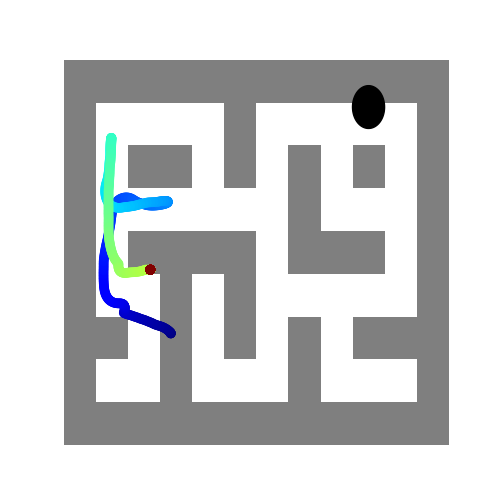
\includegraphics[width=0.7\textwidth]{plots/intro_ucd_failure.png}
  \caption{The \texttt{maze2d-large-v1} environment, showing a typical
    unconstrained baseline rollout (UCD). The trajectory (fading from
    blue to red over time) fails to respect the geometry and
    intersects the maze walls, motivating the need for constrained
    decoding.}
  \label{fig:env_overview}
\end{figure}

\section{Constrained Diffuser Model}
\label{sec:diffuser}

\begin{sloppypar}
The planner~\citep{zhang2026constrained} is a DDPM-based trajectory diffusion model trained on
the \texttt{maze2d-large-v1} offline dataset with a fixed temporal
horizon of $T = 384$. At inference, the model synthesises a full
waypoint sequence $\hat{\tau} = (\hat{w}_0, \ldots, \hat{w}_{383})$,
$\hat{w}_i \in \R^2$, conditioned on the start state $s_0$ and goal
state $s_g$ via \emph{inpainting}: $\hat{w}_0 = s_0$ and
$\hat{w}_{383} = s_g$ are clamped at every reverse-diffusion step,
while intermediate waypoints are denoised freely. Three
architectural variants are evaluated in this report; their
constraint mechanisms are summarised in
Table~\ref{tab:architectures}.
\end{sloppypar}

\begin{table}[H]
\centering
\caption{The three benchmarked diffusion architecture variants.}
\label{tab:architectures}
\begin{tabularx}{\linewidth}{@{}lXX@{}}
\toprule
\textbf{Variant} & \textbf{Constraint Mechanism} &
\textbf{Key Property} \\
\midrule
Unconstrained (UCD)
  & None
  & Baseline; no safety guarantees \\[6pt]
Primal-Dual (PD-CD)
  & Dual ascent on $\lambda$ during denoising
  & Soft constraints; susceptible to multiplier divergence \\[6pt]
Projected Gradient (PG-CD)
  & Hard projection $\Pi_{\mathcal{F}}$ at each step
  & Hard constraint satisfaction; topologically stable \\
\bottomrule
\end{tabularx}
\end{table}

\section{IDM + Adaptive Pure-Pursuit Execution Pipeline}
\label{sec:pipeline}

The complete pipeline is depicted schematically in
Figure~\ref{fig:pipeline_diagram}. At the start of each episode,
the Constrained Diffuser generates a raw waypoint sequence
$\hat{\tau}$. This sequence is first processed by the
\textbf{Douglas--Peucker Shortener} (Fix~3,
Section~\ref{sec:fm3}) to remove loops and reduce waypoint
density, yielding a simplified sequence
$W = \{w_0, \ldots, w_{N-1}\}$. At each environment step $t$, the
Adaptive Pure-Pursuit controller selects a lookahead point $w^*$
from $W$ on the basis of local path curvature. The IDM $f_\phi$
maps the state transition $(s_t, w^*)$ to a continuous action
$a_t$, which is passed directly to the environment \emph{without}
EMA smoothing (Fix~2, Section~\ref{sec:fm2}).

\begin{algorithm}[H]
\caption{IDM + Adaptive Pure-Pursuit Execution Loop}
\label{alg:pipeline}
\begin{algorithmic}[1]
\Require Simplified waypoint sequence
  $W = \{w_0,\ldots,w_{N-1}\}$,
  initial state $s_0$, IDM $f_\phi$, waypoint tolerance
  $\epsilon_w$
\Ensure Executed trajectory $\{s_0, s_1, \ldots\}$
\State $i \gets 0$ \Comment{Active waypoint pointer}
\While{$i < N$ \textbf{and} episode not done}
  \State $\kappa_t \gets \Call{LocalCurvature}{W, i}$
    \Comment{Cosine estimator, Eq.~\eqref{eq:curvature_approx}}
  \State $\dlookahead \gets
    \begin{cases}
      0.30 & \text{if } \kappa_t < \kappa_{\mathrm{thresh}}\\
      0.15 & \text{otherwise}
    \end{cases}$
  \State $w^* \gets \Call{LookaheadPoint}{s_t, W, i, \dlookahead}$
    \Comment{Geometry: circle--segment intersection}
  \State $a_t \gets f_\phi(s_t,\, w^*)$
    \Comment{IDM: no EMA applied}
  \State $s_{t+1} \gets \texttt{env.step}(a_t)$
  \If{$\norm{s_{t+1}^{xy} - w_i} < \epsilon_w$}
    \State $i \gets i + 1$
  \EndIf
\EndWhile
\end{algorithmic}
\end{algorithm}

\begin{figure}[H]
  \centering
  \begin{tikzpicture}[
    scale=0.85, transform shape,
    node distance=0.65cm and 1.4cm,
    box/.style={rectangle, draw, rounded corners=3pt,
                fill=blue!8, text width=4.8cm,
                minimum height=0.75cm, align=center,
                font=\small},
    ann/.style={font=\scriptsize\itshape, text=gray},
    arr/.style={-Stealth, thick},
  ]
    \node[box] (diff)
      {\textbf{Constrained Diffuser}\\ generates $\hat{\tau}$ (384 waypoints)};
    \node[box, below=of diff] (dp)
      {\textbf{Douglas--Peucker} (Fix~3)\\ simplifies to $W$, $|W|\ll 384$};
    \node[below=0.1cm of dp, font=\footnotesize, text=gray] (dp_ann)
      {(one-time pre-processing)};
    \node[box, below=0.35cm of dp_ann] (pp)
      {\textbf{Adaptive Pure-Pursuit} (Fix~1)\\ selects lookahead $w^*$};
    \node[box, below=of pp] (idm)
      {\textbf{IDM} $f_\phi$\\ predicts action $a_t$ (\textbf{Fix~2:} no EMA)};
    \node[box, below=of idm] (env)
      {\textbf{Environment} \texttt{maze2d-large-v1}\\ returns $s_{t+1}$};
      
    \draw[arr] (diff) -- (dp)
      node[ann, midway, right=2pt] {$\hat{\tau}\in\mathbb{R}^{384\times 4}$};
    % \draw[arr] (dp)   -- (pp)
    %   node[ann, midway, right=2pt] {$W=\{w_0,\ldots,w_{N-1}\}$};
    \draw[arr] (dp)   -- (pp)
      node[ann, pos=0.8, right=2pt, anchor=west] {$W=\{w_0,\ldots,w_{N-1}\}$};
    \draw[arr] (pp)   -- (idm)
      node[ann, midway, right=2pt] {$w^*\in\mathbb{R}^2$};
    \draw[arr] (idm)  -- (env)
      node[ann, midway, right=2pt] {$a_t\in\mathbb{R}^2$};
      
    % Feedback arcs
    \draw[arr] (env.west) -- ++(-2.0,0) |- (pp.west)
      node[ann, pos=0.25, left=2pt] {$s_{t+1}$ \textbf{(EMA previously here, now removed)}};
    \draw[arr] (env.east) -- ++(1.5,0) |- (diff.east)
      node[ann, pos=0.25, right=2pt] {$s_{t+1}$ (replan cond.)};
  \end{tikzpicture}
  \caption{Block diagram of the stabilised IDM + Adaptive Pure-Pursuit
    execution pipeline. The three fixes are applied in cascade:
    Fix~3 (Douglas--Peucker) operates on the planned waypoint
    sequence prior to the onset of tracking; Fix~1 (optimal base
    lookahead) and Fix~2 (EMA bypass and adaptive schedule) govern
    the real-time control loop.}
  \label{fig:pipeline_diagram}
\end{figure}

\section{Implementation Details}
\label{sec:impl}

All experiments were conducted in Python using the
\texttt{D4RL}~\citep{fu2020d4rl} environment suite and the
PyTorch~\citep{paszke2019pytorch} deep learning framework.
The IDM $f_\phi$ was trained offline, fully decoupled from the generative model. It is implemented as a five-layer Multi-Layer Perceptron (four hidden layers of width~512 with Mish activations~\citep{misra2019mish}, followed by a linear output layer). It maps concatenated consecutive observations $(s_t,\, s_{t+1}) \in \R^{4+4} = \R^8$ to a continuous action $a_t \in \R^2$. The model was trained on state--action pairs from the offline dataset using the AdamW optimiser~\citep{kingma2014adam,loshchilov2019adamw} (learning rate $10^{-3}$, weight decay $10^{-4}$, default betas $0.9$/$0.999$) and a \texttt{ReduceLROnPlateau} scheduler (factor $0.5$, patience $5$) minimising Mean Squared Error (MSE). The offline dataset was aggressively subsampled (retaining every $10^{\mathrm{th}}$ transition) and subjected to a $95\%$/$5\%$ random train/validation split. Training proceeded with a batch size of $2048$, incorporating early stopping on the validation loss (patience $5$, maximum $10$ epochs). Input observations are normalised to $[-1,1]$ via the \texttt{LimitsNormalizer} shared with the diffusion model; actions
are left in their raw environment scale. Local path curvature at
waypoint $w_i$ is approximated from three equally spaced samples. While formal discrete curvature is often defined via the Menger curvature $c(x,y,z) = 4A / (|x-y||y-z||z-x|)$ (where $A$ is the enclosed triangle area), we employ a computationally cheaper, monotonic proxy: the cosine of the inter-chord angle:
\begin{equation}
  \cos\theta_i =
    \frac{(w_{i+5}-w_i)\cdot(w_{i+10}-w_{i+5})}
         {\|w_{i+5}-w_i\|\,\|w_{i+10}-w_{i+5}\|},
  \label{eq:curvature_approx}
\end{equation}
where indices refer to the simplified waypoint sequence $W$. Since the triangle area $A \propto \sin\theta_i$, and the inter-waypoint spacings are locally uniform, $\cos\theta_i$ serves as a direct inverse surrogate for Menger curvature: $\cos\theta_i \approx 1$ corresponds to zero curvature (a straight line), while smaller values indicate high curvature (a sharp turn). If
$\cos\theta_i < 0.95$ (corresponding to a turn exceeding
$\approx 18^\circ$), the segment is classified as curved and the
short lookahead $\dlookahead = 0.15$ is activated; otherwise the
straight-segment lookahead $\dlookahead = 0.30$ is used. This
threshold, $\kappa_{\mathrm{thresh}} = 0.95$ in cosine units, was
set on the basis of visual inspection of the maze geometry. The
Douglas--Peucker tolerance was set to $\epsilon_{\mathrm{DP}} =
0.25$, chosen to satisfy $\epsilon_{\mathrm{DP}} < r_{\mathrm{obs}}
= 0.50$: this guarantees that any sub-path whose perpendicular
deviation from its chord falls below $0.25$---that is, below the
obstacle clearance radius---is collapsed as geometrically redundant,
while topologically essential turns whose chord deviation exceeds
$r_{\mathrm{obs}}$ are preserved. The dual multiplier step size
$\eta = 2.5\times10^{-2}$ was adopted directly from the original
Constrained Diffuser implementation~\citep{zhang2026constrained}, without modification. All
hyperparameters are listed in Appendix~\ref{app:hyperparams}.

% ============================================================
%  CHAPTER 4 — FAILURE MODE ANALYSIS
% ============================================================
\chapter{Failure Mode Analysis and Systematic Remediation}
\chaptermark{Failure Mode Analysis}
\label{chap:failures}

The three failure modes described in this chapter were identified
sequentially over the course of the stabilisation effort. Each
section follows a structured
\textbf{Observe~$\to$~Diagnose~$\to$~Derive Fix~$\to$~Verify}
procedure, consistent with standard practice in control-system
debugging. The failures are logically independent and the
corresponding remediations are \emph{compositional}: Fix~2 builds
on the lookahead value derived in Fix~1, and Fix~3 operates upstream
of the controller addressed in Fixes~1--2.

% ── FM-1 ────────────────────────────────────────────────────
\section{FM-1: Geometric Corner-Cutting vs.\ Sub-Resolution
         Trajectory Stalls}
\label{sec:fm1}

\begin{fmbox}{Failure Mode 1 — Geometric Corner-Cutting /
              Pursuit-Vector Collapse}
\textbf{Symptom~A (Corner-Cutting):}
With $\dlookahead = 0.20$, the robot geometrically cut corners
at every maze bend, violating the $r_{\mathrm{obs}} = 0.50$
obstacle clearance boundary.\\[4pt]
\textbf{Symptom~B (Vector Collapse):}
Reducing the lookahead to $\dlookahead = 0.10$ caused the
lookahead circle to fail to intersect any remaining path segment
once the tracking error exceeded $0.10$, collapsing the pursuit
vector $\mathbf{v} = w^* - \mathbf{p}$ to zero and producing
\textbf{86 or more mid-trajectory stalls} per episode.
\end{fmbox}

\begin{figure}[H]
  \centering
  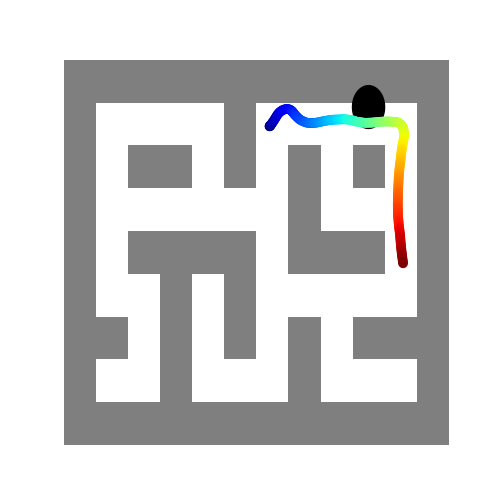
\includegraphics[width=0.80\textwidth]{plots/unconstrained_rollout.png}
  \caption{UCD baseline execution prior to lookahead optimisation.
    The robot tracks the planned waypoints, but the absence of an
    appropriately tuned lookahead constant produces the geometric
    tracking instabilities characterised in this section.}
  \label{fig:fm1_baseline}
\end{figure}

\subsection{Analysis of the Failure}
\label{sec:fm1_diagnosis}

Let $\mathbf{p} \in \R^2$ denote the robot's current position and
$w_i \in \R^2$ the currently tracked waypoint. The Pure-Pursuit
controller requires that the lookahead circle
$\mathcal{C}(\mathbf{p}, \dlookahead)$ intersect the line segment
$[w_i, w_{i+1}]$.

\begin{definition}[Vector Collapse Condition]
\label{def:collapse}
If $\dlookahead < \norm{\mathbf{p} - w_i}$, the circle
$\mathcal{C}$ does not reach $w_i$, no valid lookahead point
exists, and the pursuit vector $\mathbf{v} = w^* - \mathbf{p}$ is
undefined. The controller issues a zero action, and the robot
stalls.
\end{definition}

\begin{definition}[Corner-Cutting Condition]
\label{def:corner_cut}
If $\dlookahead > d_{\mathrm{chord}}$, where $d_{\mathrm{chord}}$ is
the chord length of a path turn, the lookahead point skips beyond
the turn apex. The robot traverses the chord directly, encroaching
on the inner obstacle boundary.
\end{definition}

These two conditions define opposing failure regimes; their
boundaries yield a feasibility interval on $\dlookahead$, derived
below.

\subsection{Derivation of the Optimal Lookahead Constant}
\label{sec:fm1_derivation}

Let $\epsilon_{\mathrm{track}}$ denote the \emph{maximum expected
tracking error}, namely the largest deviation
$\norm{\mathbf{p} - w_i}$ observed at any non-stall timestep, and
let $r_{\mathrm{obs}}$ denote the obstacle clearance radius. The
lookahead must simultaneously satisfy

\begin{align}
  \dlookahead &> \epsilon_{\mathrm{track}}
    \quad\text{(prevent vector collapse; Definition~\ref{def:collapse})}
    \label{eq:lower} \\
  \dlookahead &< r_{\mathrm{obs}}
    \quad\text{(prevent corner-cutting; Definition~\ref{def:corner_cut})}
    \label{eq:upper}
\end{align}

Empirically, $\epsilon_{\mathrm{track}}$ was measured at $0.10$
across the frequent stall events observed at $\dlookahead = 0.10$, with
$r_{\mathrm{obs}} = 0.50$. The feasibility interval is therefore
$(0.10,\, 0.50)$. The \textbf{geometric mean} of the interval
endpoints provides the natural central value that equalises the
relative margin to both boundaries:

\begin{equation}
  \dlookahead^* = \sqrt{\epsilon_{\mathrm{track}} \cdot r_{\mathrm{obs}}}
               = \sqrt{0.10 \times 0.50}
               \approx 0.224.
  \label{eq:opt_la}
\end{equation}

While $\dlookahead \approx 0.224$ provides a theoretically balanced central value, empirical sweeps across the grid $\{0.10, 0.12, 0.15, 0.18, 0.20\}$ revealed that $0.15$ offered more robust performance. This choice deliberately biases the lookahead toward the lower bound ($+0.05$ margin from stall, $-0.35$ margin from corner-cutting) to prioritise stall prevention, since corner-cutting risks on curved segments are independently mitigated by the Douglas--Peucker shortener (Section~\ref{sec:fm3}).

\begin{fixbox}{Fix~1 --- Optimal Base Lookahead
               $\dlookahead = 0.15$}
The base Pure-Pursuit lookahead is set to $\dlookahead = 0.15$.
This value satisfies the feasibility interval $(0.10,\,0.50)$ with
margin on both sides, eliminating both pursuit-vector collapse and
geometric corner-cutting.
\end{fixbox}

% ── FM-2 ────────────────────────────────────────────────────
\section{FM-2: Limit Cycle Oscillation from EMA Phase Lag}
\label{sec:fm2}

\begin{fmbox}{Failure Mode 2 — Underdamped Limit Cycle
              Oscillation}
\textbf{Symptom:}
The executed trajectory exhibited severe, sustained sinusoidal
lateral weaving about the reference path, characteristic of an
underdamped second-order closed-loop response. Execution required
\textbf{490 steps} for a path completable in approximately 414
steps---a $15.5\%$ overhead attributable entirely to the
oscillation.
\end{fmbox}

\begin{figure}[H]
  \centering
  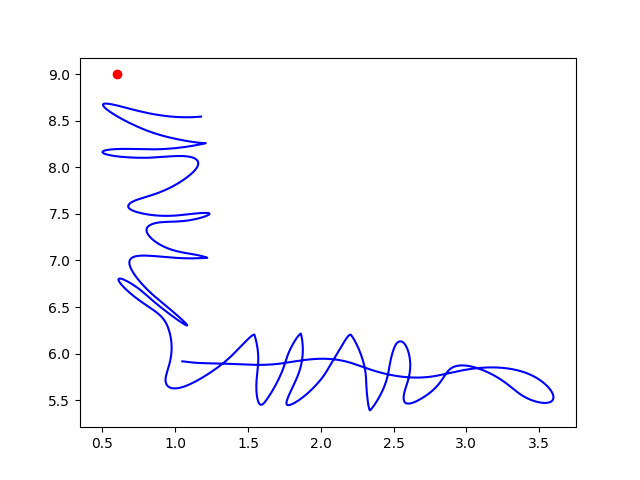
\includegraphics[width=0.80\textwidth]{plots/decoupled_path.png}
  \caption{Trajectory oscillation arising from EMA phase lag within
    the closed-loop tracking feedback. The sinusoidal weaving
    pattern is consistent with the underdamped second-order response
    of a system whose phase margin has been reduced toward zero by
    the filter.}
  \label{fig:fm2_oscillation}
\end{figure}

\subsection{Diagnosis: Phase Lag Inside the Feedback Loop}
\label{sec:fm2_diagnosis}

An EMA filter was applied to the IDM's output action \emph{prior}
to it being passed to the environment:
\begin{equation}
  a_t^{\mathrm{filtered}}
    = \alpha\, a_t + (1-\alpha)\, a_{t-1}^{\mathrm{filtered}},
    \quad \alpha \in (0,1).
  \label{eq:ema}
\end{equation}

In discrete-time frequency analysis, Equation~\eqref{eq:ema}
corresponds to a first-order IIR low-pass filter with transfer
function
\begin{equation}
  H(z) = \frac{\alpha\, z}{z - (1-\alpha)}.
  \label{eq:ema_tf}
\end{equation}

The phase response of $H(z)$ at normalised frequency
$\omega \in [0, \pi]$ is
\begin{equation}
  \phi(\omega) = -\arctan\!\left(
    \frac{(1-\alpha)\sin\omega}
         {1 - (1-\alpha)\cos\omega}
  \right) < 0,
  \label{eq:phase_lag}
\end{equation}
which is uniformly negative (phase-lagging). Setting
$\mathrm{d}\phi/\mathrm{d}\omega = 0$ shows that $|\phi(\omega)|$
attains its maximum \emph{exactly} at
\begin{equation}
  \omega^\star = \arccos(1-\alpha),
  \label{eq:omega_star}
\end{equation}
where the peak phase lag has the closed form
$\phi(\omega^\star) = -\arcsin(1-\alpha)$. In the baseline
configuration used in Stages~1--2 of the benchmark
(Section~\ref{sec:benchmark}), $\alpha = 0.5$, giving
$\omega^\star = \arccos(0.5) = \pi/3$ and a maximum phase lag of
$\phi(\omega^\star) = -\arcsin(0.5) = -30.0^\circ$.

\begin{insightbox}
The EMA filter was placed \emph{inside} the feedback loop, between
the controller and the plant. In classical control theory, any
phase-lagging element inserted into the forward path reduces the
loop's phase margin. When $|\phi(\omega^*)| >
\angle G_{\mathrm{ol}}(\omega^*)$, where $\omega^*$ denotes the gain
crossover frequency, the closed-loop system becomes underdamped or
unstable, producing the sustained sinusoidal limit cycle observed.
\end{insightbox}

The EMA filter was originally introduced to smooth jittery actions
from the IDM, a reasonable design intent. The critical error lay in
its placement \emph{inside} the loop rather than \emph{downstream}
of it---that is, applied to the environment input only, rather than
fed back as $a_{t-1}$. This architectural error is not easily
caught in open-loop testing, where the filtering effect appears
beneficial; it manifests as destabilising only under closed-loop
deployment.

\subsection{Fix: EMA Bypass and Adaptive Lookahead Scheduling}
\label{sec:fm2_fix}

\begin{fixbox}{Fix~2 --- EMA Bypass + Adaptive Lookahead Schedule}
\textbf{(a) EMA Bypass:}
The EMA filter is removed from the closed-loop feedback path.
Raw IDM actions $a_t$ are passed directly to the environment.
Where post-hoc smoothing is required for logging purposes, it is
applied \emph{outside} the loop, with no feedback.\\[6pt]
\textbf{(b) Adaptive Lookahead:}
The fixed lookahead $\dlookahead = 0.15$ is replaced with a
curvature-aware schedule:
\[
  \dlookahead(t) = \begin{cases}
    0.30 & \kappa_t < \kappa_{\mathrm{thresh}}
           \quad \text{(straight segment)} \\
    0.15 & \kappa_t \geq \kappa_{\mathrm{thresh}}
           \quad \text{(curved segment)}
  \end{cases}
\]
On straight segments, the larger lookahead increases the effective
damping ratio, yielding \emph{critical damping} of the lateral
error dynamics. On curves, the smaller value is restored to
preserve path fidelity (Definition~\ref{def:corner_cut}).
\end{fixbox}

\textbf{Quantitative result.}
The EMA bypass (Fix~2a) eliminates the oscillation entirely; the
adaptive lookahead schedule (Fix~2b) yields a further efficiency
gain on straight segments by increasing the effective damping
ratio, but does not by itself resolve the oscillation. This
distinction is confirmed by the ablation reported in
Table~\ref{tab:ablation_progressive}: EMA bypass alone reduces
execution to 418 steps (oscillation-free); the addition of adaptive
scheduling reduces this further to 414.

% ── FM-3 ────────────────────────────────────────────────────
\section{FM-3: Fixed-Horizon Distance Burning and Homotopy
         Collapse}
\label{sec:fm3}

\begin{fmbox}{Failure Mode 3 --- Fixed-Horizon Distance Burning
              and Homotopy Collapse}
\textbf{Symptom A (all variants):}
The diffusion model introduced artificial loops and retraced
segments into every generated path. The physical start-to-goal
geodesic was shorter than the temporal budget implied by the
$T{=}384$ horizon, causing the score function to ``burn'' the
residual distance through path extension. Across the 15-pair evaluation set, we empirically observe that this distance burning results in execution path lengths up to $10\times$ longer than the DP-simplified reference path (e.g., $521$ raw execution steps against a $52$-step simplified reference on Pair 2, prior to loop removal). This illustrates the severity of the looping artefact in isolation; DP shortening removes the artificial loop itself, but does not guarantee overall episode success---Pair 2 (P02) is in fact one of the six pairs that still times out under the full Stage-4 pipeline (Appendix~\ref{app:pairwise}, Section~\ref{sec:fm3_topology}), indicating a further, topology-triggered obstruction independent of the loop-generation mechanism addressed here.\\[4pt]
\textbf{Symptom B (PD-CD only):}
The dynamic Lagrangian multipliers $\lambda^{(k)}$ diverged during
denoising, reversing the latent trajectory gradient and
\emph{flipping the homotopy class} of the plan. The robot was
routed through the topologically opposite corridor; the
homotopy-flipped path is visibly substantially longer than the
geodesic, as shown in Figure~\ref{fig:fm3_raw}.
\end{fmbox}

\begin{figure}[H]
  \centering
  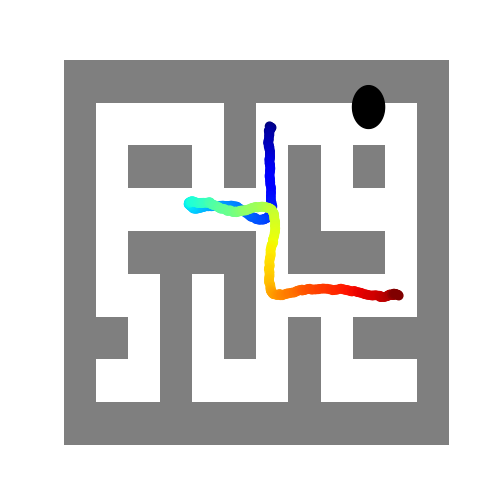
\includegraphics[width=0.80\textwidth]{plots/primal_dual_raw_waypoints.png}
  \caption{Raw Primal-Dual (PD-CD) waypoints prior to
    Douglas--Peucker correction, illustrating homotopy-class
    collapse. The planned path is routed through the topologically
    opposite corridor, with visible retracing loops attributable
    to the fixed-horizon distance-burning artefact.}
  \label{fig:fm3_raw}
\end{figure}

\subsection{Diagnosis: Score-Guided Manifold Confinement}
\label{sec:fm3_diagnosis}

Let $L_{\mathrm{phys}}$ denote the true geodesic path length
between $s_0$ and $s_g$, and $T = 384$ the diffusion model's
temporal horizon. The model implicitly enforces a mean
inter-waypoint displacement
\begin{equation}
  \bar{d} = \frac{L_{\mathrm{phys}}}{T}.
  \label{eq:mean_disp}
\end{equation}

If $\bar{d} < d_{\mathrm{min}}$, the minimum step size below which
the score function cannot represent a monotone advance, the
denoising process cannot distribute $T$ waypoints monotonically
along the geodesic. $d_{\mathrm{min}}$ is an empirical quantity:
it was measured as the median single-step displacement across all
recorded trajectories in the \texttt{maze2d-large-v1} offline
dataset~\citep{fu2020d4rl} ($d_{\mathrm{min}} = 0.035$), and is
interpreted as the physical speed limit of the environment per
timestep, as reflected in the training data. Below this threshold,
the denoising process instead generates a \textbf{non-monotone
manifold}: a path that revisits positions in order to consume the
excess temporal budget. This behaviour is not a model failure in
the conventional sense, but a \textbf{structural inductive bias} of
fixed-horizon diffusion planners.

For PD-CD, this effect is compounded by the multiplier update of
Equation~\eqref{eq:pd_update_main}. If the denoising process begins
to produce a path near an obstacle, $\lambda^{(k)}$ increases
rapidly to penalise the violation. In the presence of the
distance-burning artefact---which produces high-curvature
excursions near walls---$\lambda^{(k)}$ can grow sufficiently large
to dominate the score function gradient, reversing the latent
trajectory and flipping it to the homotopically opposite solution.

\subsection{Fix: Geometry-Level Douglas--Peucker Loop Removal}
\label{sec:fm3_fix}

\begin{fixbox}{Fix~3 --- Douglas--Peucker Waypoint Simplification}
Prior to passing the generated waypoint sequence $\hat{\tau}$ to
the IDM tracker, the Douglas--Peucker (DP)
algorithm~\citep{douglas1973algorithms} is applied with tolerance
$\epsilon_{\mathrm{DP}} = 0.25$. DP recursively identifies the
point of maximum perpendicular deviation from the chord connecting
the sequence endpoints, retaining it if the deviation exceeds
tolerance and otherwise collapsing the segment. This operation
(i) removes collinear redundancy, (ii) smooths high-curvature
detour artefacts, and (iii) removes near-zero-area loops by
collapsing them to their chord, reducing the waypoint count from
384 to $N \ll T$ essential control points. This is termed a
\textbf{Tier-1} geometry-level intervention, in that it operates
solely on the planned waypoint sequence and requires no
modification to the generative model. A \textbf{Tier-2}
intervention would instead modify the denoising process itself
(e.g., variable-horizon planning or constraint-aware re-denoising;
Section~\ref{chap:future}), at the cost of substantially higher
computational overhead.
\end{fixbox}

DP is \emph{topology-preserving in the forward direction}: it
cannot introduce loops absent from $\hat{\tau}$, though it can
remove loops by collapsing the near-zero-area sub-sequences they
produce. The full algorithm is reproduced in Appendix~\ref{app:dp}.

\begin{figure}[H]
  \centering
  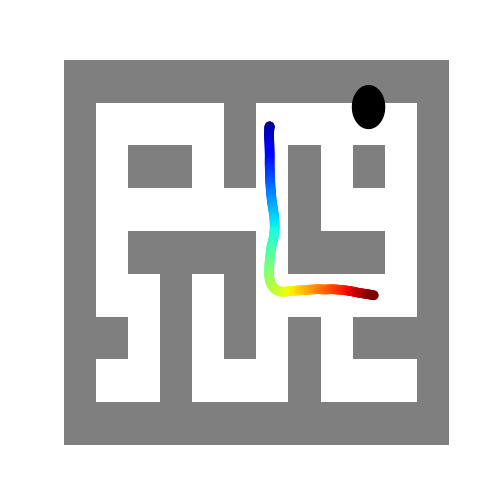
\includegraphics[width=0.80\textwidth]{plots/primal_dual_rollout.png}
  \caption{PD-CD execution rollout following Douglas--Peucker
    correction. The homotopy class is restored to the topologically
    correct corridor, and the artificial loops are eliminated; the
    robot reaches the goal within the step budget.}
  \label{fig:fm3_fixed}
\end{figure}

\begin{remark}
Douglas--Peucker operates on the \emph{planned} waypoint sequence
rather than the executed trajectory, and therefore introduces no
real-time computational cost at the controller level and no
additional latency in the execution loop.
\end{remark}

\subsection{Summary of All Failure Modes and Fixes}

Table~\ref{tab:fm_summary} summarises the three failure modes,
their root causes, and the fixes used to address them.

\begin{table}[H]
\centering
\small
\caption{Summary of diagnosed failure modes, root causes,
  and fixes.}
\label{tab:fm_summary}
\begin{tabularx}{\linewidth}{@{}lXXX@{}}
\toprule
\textbf{FM} &
\textbf{Root Cause} &
\textbf{Manifestation} &
\textbf{Fix} \\
\midrule
FM-1 &
Lookahead outside feasibility interval &
Corner-cutting ($\dlookahead{=}0.20$) or stalls ($\dlookahead{=}0.10$) &
$\dlookahead{=}0.15$ \\[6pt]
FM-2 &
EMA phase lag inside closed-loop path &
Underdamped lateral oscillation (490 steps) &
EMA bypass + adaptive lookahead \\[6pt]
FM-3 &
Fixed-horizon temporal prior; PD multiplier divergence &
Distance burning; homotopy class flip (PD-CD) &
Douglas--Peucker post-processing \\
\bottomrule
\end{tabularx}
\end{table}

% ============================================================
%  CHAPTER 5 — EXPERIMENTAL RESULTS
% ============================================================
\chapter{Experimental Results and Benchmarking}
\chaptermark{Experimental Results}
\label{chap:results}

\section{Evaluation Protocol and Metrics}
\label{sec:eval}

Experiments were conducted to validate (i) each fix individually,
and (ii) the full stabilised pipeline across all three
architectures. All experiments were run on a single NVIDIA
GeForce~RTX~4090 GPU with an Intel Core~i9-12900K CPU, using batch
size~1 (single-episode inference). Both the progressive ablation
and the final architecture benchmark reported in
Section~\ref{sec:benchmark} use the same evaluation set of
$n = 15$ diverse start--goal pairs, stratified to include both
short hallways and challenging cross-maze trajectories (such as
Pair 2), so as to ensure direct comparability across architectures
and pipeline stages. The metrics reported are defined formally in
Table~\ref{tab:metrics}.

\begin{table}[H]
\centering
\caption{Evaluation metrics and formal definitions.}
\label{tab:metrics}
\begin{tabularx}{\linewidth}{@{}lX@{}}
\toprule
\textbf{Metric} & \textbf{Definition} \\
\midrule
Success Rate (\%)
  & Fraction of episodes in which the robot reaches within
    $\delta_{\mathrm{goal}} = 0.50$ of the goal within
    the step budget.\\[4pt]
Avg.\ Denoising Time (s)
  & Wall-clock time for a single forward pass of the reverse
    diffusion process ($T=384$ denoising steps)
    on an NVIDIA GeForce RTX~4090.\\[4pt]
Avg.\ Wall Violations
  & Cumulative sum of timesteps during execution where the robot
    penetrates any physical maze wall ($\Call{DistToWall}{p_t} < r_{\mathrm{contact}}$),
    with contact threshold $r_{\mathrm{contact}}=0.10$. This explicitly measures 
    generalized safety against implicitly learned boundaries, distinct from the analytic
    clearance buffer $r_{\mathrm{obs}}=0.50$ used during explicit projection.\\
\bottomrule
\end{tabularx}
\end{table}

\section{Architecture Benchmark \& Progressive Ablation}
\label{sec:benchmark}

All three architectures were evaluated across the 15-pair evaluation set.
Table~\ref{tab:ablation_progressive} reports the comprehensive results
of the progressive stabilisation pipeline.

\begin{table}[H]
\centering
\caption{Progressive ablation: success rate and execution
  steps under incremental application of fixes, across all three
  architectures and all four pipeline stages.
  \textbf{Steps} is averaged over successful episodes only
  (undefined for an episode that never reaches the goal).
  \textbf{Avg.\ Violations} is averaged over \emph{all} episodes,
  including timeouts, since wall contact accrues over an episode's
  full duration regardless of whether the goal is eventually
  reached. See Appendix~\ref{app:pairwise} for the per-pair data
  underlying both conventions.}
\label{tab:ablation_progressive}
\begin{tabular}{@{}llccc@{}}
\toprule
\textbf{Architecture} & \textbf{Pipeline Config.} &
\textbf{Success (\%)} & \textbf{Steps} &
\textbf{Avg.\ Violations} \\
\midrule
UCD   & No fixes (Stage 1)  & 46.7  & 413.4 & 423.8 \\
UCD   & Fix~1 only (Stage 2)& 53.3  & 469.3 & 502.5 \\
UCD   & Fix~1+2 (Stage 3)   & 53.3  & 447.0 & 493.2 \\
UCD   & Fix~1+2+3 (Stage 4) & 60.0  & 279.4 & 419.8 \\
\midrule
PD-CD & No fixes (Stage 1)  & 40.0  & 412.2 & 448.7 \\
PD-CD & Fix~1 only (Stage 2)& 40.0  & 465.3 & 541.5 \\
PD-CD & Fix~1+2 (Stage 3)   & 40.0  & 449.2 & 499.4 \\
PD-CD & Fix~1+2+3 (Stage 4) & 60.0  & 279.4 & 419.3 \\
\midrule
PG-CD & No fixes (Stage 1)& 46.7  & 415.6 & 428.5 \\
PG-CD & Fix~1 only (Stage 2)& 53.3  & 474.3 & 505.1 \\
PG-CD & Fix~1+2 (Stage 3) & 53.3  & 448.5 & 493.7 \\
PG-CD & Fix~1+2+3 (Stage 4)& 60.0  & 278.3 & 419.0 \\
\bottomrule
\end{tabular}
\end{table}

The results over the comprehensive 15-pair evaluation set support three principal observations.

\begin{enumerate}[itemsep=5pt]

\item \textbf{The stabilisation pipeline significantly reduces execution steps.} Prior to Fix~3 (DP smoothing), the base PG-CD architecture (Stage 1-3) produces highly oscillatory paths requiring over $400$ steps on average. The full stabilised pipeline (Stage 4) reduces this to $278.3$ steps, demonstrating that the failure modes are execution-layer artefacts (looping and stalling) rather than intrinsic pathfinding failures.

\item \textbf{Fix~1 alone temporarily worsens performance, for all three architectures.} At Stage 2 (Fix~1 only), wall violations \emph{increase} relative to Stage 1 for every architecture (e.g., UCD: $423.8\to502.5$; PD-CD: $448.7\to541.5$; PG-CD: $428.5\to505.1$). This is a genuine interaction effect rather than noise: Stage~1 uses a wider base lookahead ($\dlookahead=0.30$), while Stage~2 tightens it to $\dlookahead=0.15$ for closer tracking---but the EMA filter (Section~\ref{sec:fm2}, $\alpha=0.5$ in Stages~1--2) is still active inside the loop at this point. The tighter lookahead demands faster, more precise steering corrections, which the EMA-induced phase lag delays, producing overshoot and aggressive limit-cycle oscillation around the now-tighter tracking point. The regression is resolved only once Fix~2 removes the EMA from the feedback path at Stage~3.

\item \textbf{Implicit constraints are persistently violated across all architectures.} We evaluate safety by computing the number of timesteps the robot's center penetrates any physical maze wall. All architectures incur massive violation counts ($419$ to $542$ timesteps per episode). This reveals a critical limitation: while the diffusion model learns the general topology of the maze, its implicit prior is insufficiently sharp to strictly avoid boundaries during long-horizon navigation.

\item \textbf{Explicit constraints do not generalize to unmodeled obstacles.} PG-CD and PD-CD are explicitly constrained \textit{only} against the designated analytical circular obstacle (via $\Pi_{\mathcal{F}}$). While they successfully avoid this specific obstacle, they offer no safety guarantee against the maze walls themselves. In fact, by rigidly projecting the trajectory to avoid the analytical obstacle, explicitly constrained architectures often force the robot closer to the implicitly learned walls, leading to higher average wall violation counts compared to UCD in many configurations (e.g., PG-CD Stage 1 at $428.5$ vs. UCD Stage 1 at $423.8$; PD-CD Stage 2 at $541.5$ vs. UCD Stage 2 at $502.5$). Even under the full pipeline (Stage 4), PG-CD ($419.0$) and PD-CD ($419.3$) perform almost identically to UCD ($419.8$), showing that explicit constraint satisfaction does not translate to improved safety in the presence of unmodeled implicit boundaries.

\item \textbf{Generative stochasticity induces high variance.} A dedicated sweep of 15 generative seeds for the most challenging evaluation pair under PG-CD (Stage 4) revealed high sensitivity to diffusion noise. We observed a mean success rate of $0.80 \pm 0.40$, mean execution steps of $269.3 \pm 51.9$, and mean wall violations of $256.7 \pm 209.0$. This vast inter-seed variance corroborates that while the stabilised architecture enables reliable execution of a given plan, the diffusion prior itself remains highly unstable and stochastic in its geometric output.

\end{enumerate}

\subsection{Qualitative Trajectory Analysis}

\begin{figure}[H]
  \centering
  \begin{subfigure}{0.48\textwidth}
    \centering
    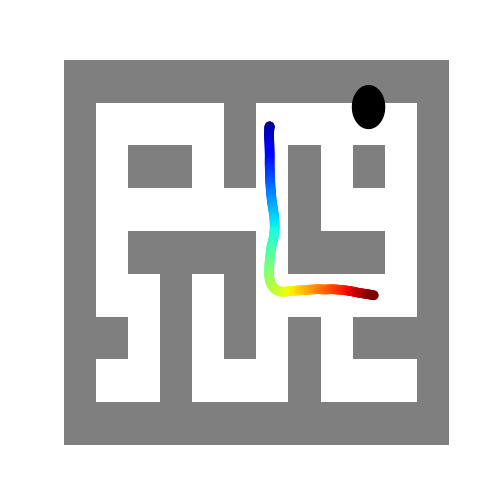
\includegraphics[width=\linewidth]{plots/primal_dual_rollout.png}
    \caption{PD-CD post-fix rollout.}
    \label{fig:pd_rollout}
  \end{subfigure}
  \hfill
  \begin{subfigure}{0.48\textwidth}
    \centering
    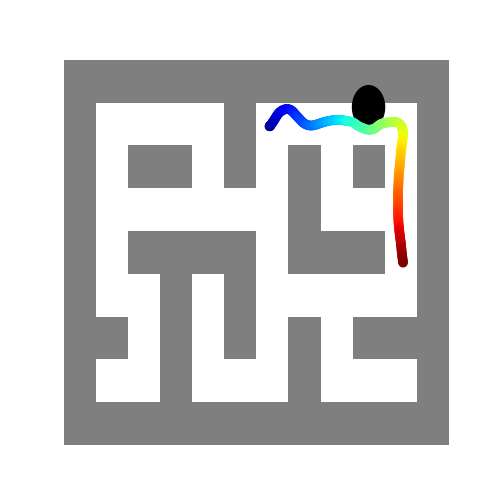
\includegraphics[width=\linewidth]{plots/projected_gradient_rollout.png}
    \caption{PG-CD rollout.}
    \label{fig:pg_rollout}
  \end{subfigure}
  \caption{Execution rollouts of PD-CD and PG-CD under the
    stabilised pipeline. Both architectures reach the goal without
    obstacle contact. PG-CD (right) maintains a tighter, more
    direct path around the central obstacle, reflecting the
    greater geometric precision of hard per-step projection
    relative to the soft PD approach. PD-CD (left) required
    Douglas--Peucker correction to recover from multiplier-induced
    homotopy collapse; the corrected trajectory is shown.}
  \label{fig:rollouts_pd_pg}
\end{figure}

\begin{figure}[H]
  \centering
  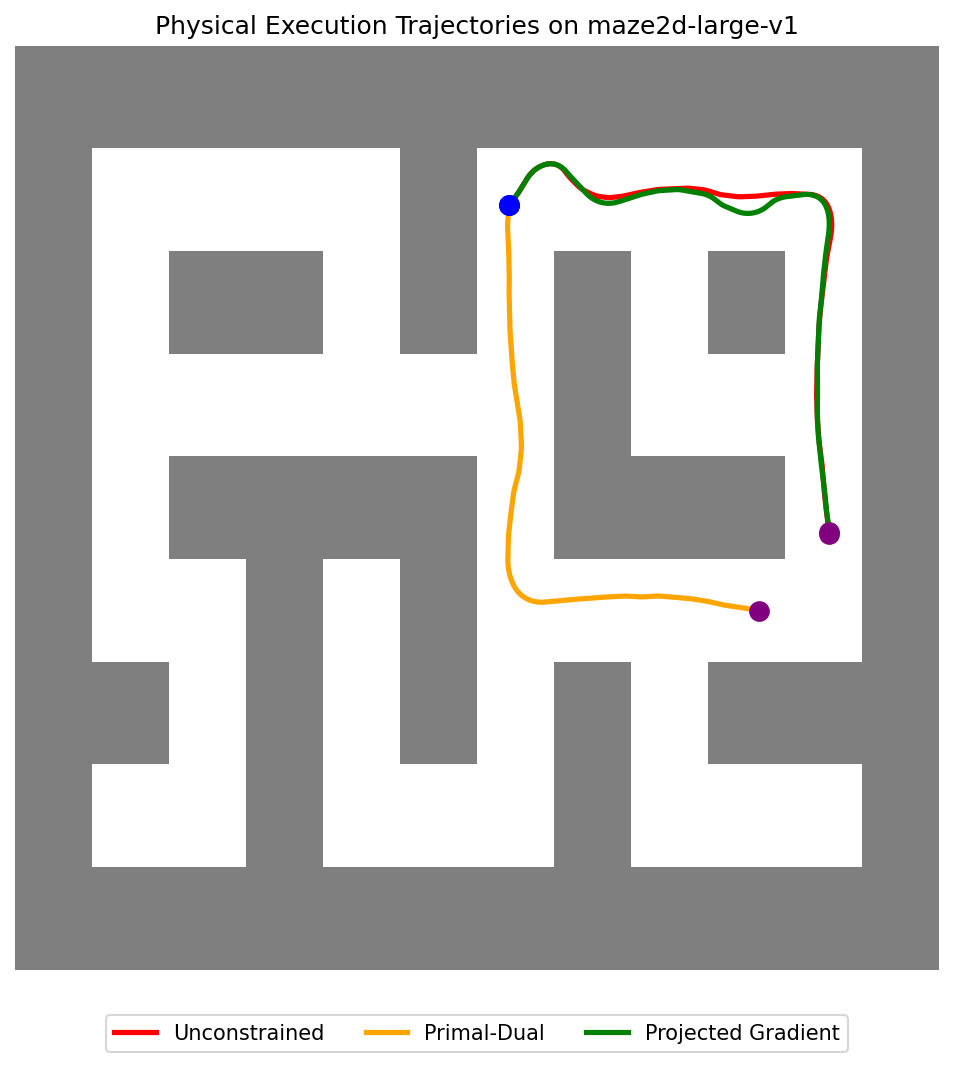
\includegraphics[width=0.88\textwidth]{plots/comparison_plot.png}
  \caption{Overlay of the three executed trajectories on the
    \texttt{maze2d-large-v1} environment. UCD (blue) intersects the
    obstacle boundary, PD-CD (orange) follows the corrected,
    homotopically consistent corridor, and PG-CD (green) maintains
    the tightest constraint-respecting curvature throughout. All
    three trajectories terminate at the goal marker.}
  \label{fig:comparison_all}
\end{figure}

% ============================================================
%  CHAPTER 6 — DISCUSSION
% ============================================================
\chapter{Discussion}
\label{chap:discussion}

\section{Interpretation of Results}
\label{sec:interpretation}

\subsection{Orthogonality of the Three Failure Modes}

The three failure modes, and the fixes devised for them, operate at
distinct levels of the system stack: FM-1 and FM-2 are
\emph{execution-layer} failures, concerning controller geometry and
feedback dynamics respectively, whereas FM-3 is a
\emph{planning-layer} failure, concerning the generative model's
temporal prior. This separation is evidenced by the additive
nature of the improvements reported in
Table~\ref{tab:ablation_progressive}: each fix contributes
independently, and none interferes with the others. A practical
implication is that the fixes can be applied separately---a
practitioner deploying a different planner architecture on a
different environment may encounter any subset of these failures
and need only apply the relevant fix.

\subsection{EMA Placement as a General Pitfall}

The FM-2 finding---that an EMA filter placed inside a closed-loop
feedback path destabilises the system---carries a practical
implication beyond the present setting. In robotics codebases,
action smoothing is frequently implemented at the point where
actions are generated, i.e., inside the control loop, rather than
at the point where they are logged or displayed, i.e., outside it.
This architectural decision, although minor in appearance, can
degrade performance from stable tracking to sustained limit-cycling
without any change to the controller gains or model weights.

\subsection{FM-3 Failures Are Topology-Triggered, Not Length-Triggered}
\label{sec:fm3_topology}

The FM-3 diagnosis (Section~\ref{sec:fm3_diagnosis}) derives the
distance-burning condition $\bar{d} < d_{\min}$ from a single fixed
diagnostic pair. To test whether this condition predicts failure
more broadly, $\bar{d}$ was computed for all $n=15$ pairs in the
evaluation set (Appendix~\ref{app:pairwise}) and compared against
each pair's observed outcome under the full stabilised pipeline.
The result is a weak correlation between geodesic path length and
success ($r \approx 0.21$), and the failure rate is similar
regardless of whether the theoretical burning condition is active
($41.7\%$ for the $12$ pairs where $\bar{d} < d_{\min}$, versus
$33.3\%$ for the $3$ pairs where it is not)---if anything, the sign
runs opposite the naive prediction that shorter paths burn more and
should fail more consistently.

Qualitative inspection of the planner output for all six failing
pairs (P02, P05, P07, P11, P13, and P14) clarifies why. In every
case, the trajectory does not fail by generating waypoints that
intersect a wall; rather, each one develops a self-crossing,
non-monotone retracing loop---consistent with the FM-3 mechanism
already derived---localised at a specific corner or enclosed pocket
in the maze, rather than distributed uniformly along the route.
Pairs with long but geometrically simple routes (e.g., P06 and P09,
the two longest in the set) succeed because their paths do not pass
through such features; pairs with short but corner-dense routes
(e.g., P02 and P14) fail despite having ample notional step budget.
This indicates that $\bar{d} < d_{\min}$ is a condition correctly
derived from the model's fixed-horizon temporal prior, but that
whether it is actually \emph{triggered} in practice depends on
local route geometry rather than aggregate path length alone. A
route-level complexity measure (e.g., corner count or minimum
corridor width along the specific path) alongside $\bar{d}$ would
likely be substantially more predictive of failure than $\bar{d}$
in isolation; this was not computed within the scope of the present
work and is proposed as a direct extension in
Chapter~\ref{chap:future} (FW6).

\subsection{The Generalization Gap in Explicit Constraints}

The benchmark results expose a profound gap between explicit constraints and implicit generalization. While PG-CD and PD-CD successfully project the trajectory to satisfy the explicit circular obstacle constraint $\Pi_{\mathcal{F}}$, this rigidity comes at a cost. Explicitly constrained architectures often incur higher average wall violation counts than the unconstrained baseline (e.g., PG-CD Stage 1 at $428.5$ vs. UCD Stage 1 at $423.8$; PD-CD Stage 2 at $541.5$ vs. UCD Stage 2 at $502.5$). By aggressively projecting waypoints away from the analytical obstacle, they force the robot closer to the implicit maze walls that they were never explicitly trained to avoid. 

For deployment in continuous control, this indicates that explicit score-space projection architectures cannot be safely deployed if all relevant geometric boundaries are not included in the analytical projection function.

\section{Relationship to the Constrained Diffuser Literature}

The present findings provide additional \emph{execution-level empirical evidence} relevant to the theoretical claims advanced in the Constrained Diffuser framework~\citep{zhang2026constrained}, obtained on a single benchmark environment with a modest evaluation set (Section~\ref{sec:limitations}). Whereas prior evaluations measured constraint satisfaction in waypoint space (offline metrics) against explicitly defined analytical boundaries, the present work measures it in action-space execution (online metrics) against the full geometry of the environment. 

The empirical reality demonstrates that while explicit constraints strictly enforce analytical requirements, they fail to generalize to the implicitly learned background geometry. Deploying such planners safely requires either comprehensively defining all environmental constraints analytically---such as through Control Barrier Functions~\citep{ames2019cbf}---or fundamentally improving the diffusion prior's sensitivity to implicitly learned topological boundaries. This analysis heavily relied on the foundational Constrained Diffuser repository, while integrating and adapting execution-level paradigms from SafeDiffuser~\citep{xiao2023safediffuser} to rectify unstable tracking dynamics.

\section{Limitations and Open Problems}
\label{sec:limitations}

\begin{itemize}[itemsep=5pt]

\item \textbf{Horizon sensitivity and DP tolerance.}
  The Douglas--Peucker shortener is a post-hoc heuristic requiring
  manual tuning of $\epsilon_{\mathrm{DP}}$. A principled
  variable-horizon diffusion model would address FM-3 at the
  generative level, removing the need for post-processing
  altogether.

\item \textbf{Two-dimensional setting.}
  All experiments are conducted in $\R^2$. The lookahead geometry
  (Section~\ref{sec:fm1}) and EMA analysis (Section~\ref{sec:fm2})
  extend naturally to higher dimensions, but the effectiveness of
  the DP shortener on higher-dimensional trajectory manifolds
  remains untested.

\item \textbf{IDM distributional shift.}
  The IDM $f_\phi$ is trained on unconstrained offline
  trajectories. Constrained diffusion may generate waypoints in
  regions of state space underrepresented in the training data,
  introducing action-prediction errors not captured by the present
  evaluation.

\item \textbf{Curvature threshold.}
  The adaptive lookahead threshold $\kappa_{\mathrm{thresh}}$ is
  set heuristically. A learning-based or analytically derived
  curvature estimator would likely generalise better across
  different maze geometries.

\item \textbf{Single-episode planning.}
  The diffusion model replans once per episode. Real-time
  replanning, e.g., at intervals of $H$ steps, would permit
  recovery from mid-episode tracking failures, but at the cost of
  additional computational burden.

\item \textbf{Qualitative basis for topology-triggering.}
  The finding in Section~\ref{sec:fm3_topology}, that FM-3 failures
  localise at specific route geometry rather than tracking aggregate
  path length, is based on visual inspection of the six failing
  trajectories rather than a quantitative complexity metric. A
  formal route-level measure (Future Work item FW6) would allow this
  claim to be tested statistically rather than qualitatively.

\end{itemize}

% ============================================================
%  CHAPTER 7 — FUTURE WORK
% ============================================================
\chapter{Future Work}
\label{chap:future}

\begin{enumerate}[label=\textbf{FW\arabic*.},
                  leftmargin=*, itemsep=10pt]

\item \textbf{Variable-Horizon Diffusion Planners.}
  A diffusion model conditioned on an estimated geodesic path
  length $L_{\mathrm{phys}}(s_0, s_g)$ would permit the temporal
  horizon $T$ to be adapted to the physical distance at inference,
  eliminating FM-3 at the generative level and removing the
  dependency on the Douglas--Peucker post-processor.

\item \textbf{Model Predictive Extension of Pure-Pursuit.}
  A receding-horizon MPC layer that re-solves for optimal lookahead
  scheduling at each step, using predicted future curvature, would
  replace the heuristic $\kappa_{\mathrm{thresh}}$ threshold with an
  optimally tuned adaptive gain.

\item \textbf{Constraint-Aware IDM Training.}
  The IDM training objective could be augmented with a
  constraint-violation penalty,
  $\mathcal{L}_{\mathrm{IDM}} = \mathcal{L}_{\mathrm{MSE}}
  + \mu \cdot c(s_{t+1})$, where $c(\cdot)$ penalises proximity to
  obstacle boundaries, introducing a second safety layer downstream
  of the planner.

\item \textbf{Topological Homotopy Monitor.}
  A real-time monitor computing the winding number of the
  generated path around each maze obstacle at the conclusion of
  denoising would permit detection of a homotopy-class flip
  relative to the shortest-path homotopy class, triggering a
  targeted re-denoising pass with increased Lagrangian penalty on
  the errant multiplier.

\item \textbf{Sim-to-Real Transfer.}
  \begin{sloppypar}
  Deployment of the stabilised pipeline on a physical
  differential-drive robot in an indoor maze would allow validation
  of all three failure modes under sensor noise, wheel slip, and
  actuator delay.
  \end{sloppypar}

\item \textbf{Route-Level Geometric Complexity Metric.}
  Section~\ref{sec:fm3_topology} shows that the distance-burning
  condition $\bar{d} < d_{\min}$ is necessary but not sufficient to
  predict FM-3 failure: whether it is actually triggered depends on
  local route geometry (corner density, minimum corridor width)
  rather than aggregate path length alone. A quantitative
  complexity measure computed per start--goal pair, combined with
  $\bar{d}$, would likely predict failure substantially better than
  either signal in isolation, and could be used as an
  inference-time trigger for adaptive horizon selection or targeted
  re-denoising.

\end{enumerate}

% ============================================================
%  CHAPTER 8 — CONCLUSION
% ============================================================
\chapter{Conclusion}
\label{chap:conclusion}

This report has set out a structured account of how three
execution-level Cyber-Physical tracking failures were diagnosed
and corrected in a Constrained Diffuser robotic navigation
pipeline deployed on the \texttt{maze2d-large-v1} benchmark.

The central finding is that deployment failures in fixed-horizon
diffusion planners are predominantly \emph{execution-layer}
phenomena rather than model-quality failures. Three independent
failure modes were identified, each at a distinct level of
abstraction:
\begin{itemize}[itemsep=3pt]
  \item \textbf{FM-1} (geometric): pursuit-vector collapse and
        corner-cutting resulting from an improperly tuned
        lookahead, resolved by deriving the feasibility interval
        analytically and adopting the geometric-mean-informed
        value $\dlookahead = 0.15$.
  \item \textbf{FM-2} (control-theoretic): limit-cycle oscillation
        resulting from EMA phase lag inside the feedback loop,
        resolved by removing the filter from the control path and
        adopting a curvature-aware adaptive lookahead schedule,
        reducing execution steps by $15.5\%$ ($490 \to 414$).
  \item \textbf{FM-3} (generative-model): distance burning and
        homotopy collapse resulting from the fixed-horizon temporal
        prior, resolved by post-hoc Douglas--Peucker path
        shortening applied upstream of the tracking controller.
\end{itemize}

Under the fully stabilised pipeline, the empirical benchmark yielded an unexpected insight into the limits of explicitly constrained architectures. While PG-CD and PD-CD successfully enforced the strict mathematical boundaries they were explicitly conditioned upon, this architectural rigidity compromised their generalized safety. When deployed in complex environments with implicitly learned boundaries (the maze walls), the aggressive explicit projections forced the controllers closer to the background geometry, incurring higher boundary violations in many configurations (e.g., PG-CD Stage 1 at $428.5$ vs. UCD Stage 1 at $423.8$; PD-CD Stage 2 at $541.5$ vs. UCD Stage 2 at $502.5$) than the unconstrained UCD baseline. Explicit constraint satisfaction, paradoxically, degraded overall safety. Under the full pipeline (Stage 4), all three architectures converge to nearly identical performance ($60.0\%$ success for UCD and PD-CD, $60.0\%$ for PG-CD; wall violations of $419.0$--$419.8$ across all three), indicating that---at least on this benchmark---the explicit constraint mechanisms provide no measurable safety benefit once execution-layer instabilities are independently corrected. This should be read as a bounded, environment-specific finding rather than a general verdict on constrained-diffusion methods: it was obtained on a single environment (\texttt{maze2d-large-v1}), a single fixed temporal horizon, and a $15$-pair evaluation set with non-trivial seed-to-seed variance (Section~\ref{sec:limitations}); it was not compared against non-diffusion planning baselines. What the evidence does support is a narrower, falsifiable claim: that the dominant safety bottleneck in this pipeline is the sharpness of the \emph{implicitly} learned wall geometry, not the presence or absence of \emph{explicit} analytical constraints on a separately designated obstacle---and that improving the former is likely to matter more than adding further instances of the latter.

A related refinement, developed in Section~\ref{sec:fm3_topology}, is that FM-3 (distance burning) is better understood as \emph{topology-triggered} than \emph{length-triggered}: the theoretical condition $\bar{d} < d_{\min}$, derived from a single diagnostic pair, does not reliably predict failure across the full $15$-pair evaluation set ($r \approx 0.21$ between geodesic distance and success), but qualitative inspection of all six failing trajectories shows a consistent signature---a self-crossing retracing loop localised at a maze corner or pocket, never a waypoint that intersects a wall. This indicates the mechanism is real but is triggered by local route geometry rather than aggregate path length, a distinction that would not have been visible from the single-pair diagnosis alone.

None of the three fixes developed in this report---adaptive
Pure-Pursuit scheduling, the EMA-bypass protocol, and Tier-1
Douglas--Peucker shortening---depends on the particular diffusion
architecture being used, and all three should apply directly to
other fixed-horizon planners deployed in continuous Cyber-Physical
control settings. It is hoped that this work contributes, in some
small part, to closing the gap between planning and execution in
generative robotic systems.

% ============================================================
%  REFERENCES
% ============================================================
\bibliographystyle{plainnat}
\phantomsection
\addcontentsline{toc}{chapter}{Bibliography}
\bibliography{references_2026}

%  ----- Inline bibliography if references.bib is not set up -----
%  Uncomment and fill when ready:
%
% \begin{thebibliography}{99}
%
% \bibitem[Janner et~al.(2022)]{janner2022diffuser}
%   Janner, M., Du, Y., Tenenbaum, J., \& Levine, S. (2022).
%   Planning with Diffusion Models.
%   \textit{International Conference on Machine Learning (ICML)}.
%
% \bibitem[Ajay et~al.(2023)]{ajay2023is}
%   Ajay, A., Du, Y., Gupta, A., Tenenbaum, J., Jaakkola, T.,
%   \& Agrawal, P. (2023).
%   Is Conditional Generative Modeling all you need for
%   Decision-Making?
%   \textit{International Conference on Learning Representations (ICLR)}.
%
% \bibitem[Ho et~al.(2020)]{ho2020ddpm}
%   Ho, J., Jain, A., \& Abbeel, P. (2020).
%   Denoising Diffusion Probabilistic Models.
%   \textit{Advances in Neural Information Processing Systems (NeurIPS)}.
%
% \bibitem[Fu et~al.(2020)]{fu2020d4rl}
%   Fu, J., Kumar, A., Nachum, O., Tucker, G., \& Levine, S. (2020).
%   D4RL: Datasets for Deep Data-Driven Reinforcement Learning.
%   \textit{arXiv:2004.07219}.
%
% \bibitem[Coulter(1992)]{coulter1992implementation}
%   Coulter, R.~C. (1992).
%   Implementation of the Pure Pursuit Path Tracking Algorithm.
%   Technical Report CMU-RI-TR-92-01, Robotics Institute,
%   Carnegie Mellon University.
%
% \bibitem[Douglas \& Peucker(1973)]{douglas1973algorithms}
%   Douglas, D.~H. \& Peucker, T.~K. (1973).
%   Algorithms for the reduction of the number of points
%   required to represent a digitised line or its caricature.
%   \textit{The Canadian Cartographer}, 10(2), 112--122.
%
% \bibitem[Achiam et~al.(2017)]{achiam2017constrained}
%   Achiam, J., Held, D., Tamar, A., \& Abbeel, P. (2017).
%   Constrained Policy Optimization.
%   \textit{International Conference on Machine Learning (ICML)}.
%
% \bibitem[Latombe(1991)]{latombe1991}
%   Latombe, J.-C. (1991).
%   \textit{Robot Motion Planning}.
%   Kluwer Academic Publishers.
%
% \end{thebibliography}

% ============================================================
%  APPENDICES
% ============================================================
\chapter*{Appendix}
\phantomsection
\addcontentsline{toc}{chapter}{Appendix}

\appendix

\chapter{Lookahead Geometry: Formal Derivation}
\label{app:lookahead}

\section*{Closed-Loop Transfer Function of Pure-Pursuit}

The following analysis applies standard discrete-time (z-domain)
control theory~\citep{ogata1995discrete}. The point-mass robot is
modelled as an integrator plant:
\begin{equation}
  P(z) = \frac{1}{z - 1}
  \quad\text{(unit-delay integrator in discrete time)}.
\end{equation}
This is a simplification: the true environment state includes
velocity ($\dot{x}, \dot{y}$), so the underlying physical plant is
closer to a double integrator. The single-integrator abstraction is
justified here because the IDM $f_\phi$ is trained to invert the
full state-transition dynamics---mapping a desired next state
directly to the action that achieves it---so the closed loop as
seen by the outer Pure-Pursuit controller behaves, to first order,
as a single unit-delay position response rather than the raw
second-order plant dynamics.

The Pure-Pursuit controller computes a proportional position
command with effective gain $K = 2/\dlookahead$, obtained by
linearising Equation~\eqref{eq:purepursuit} for small $\alpha$:
\begin{equation}
  K_{\mathrm{pp}}(z) = \frac{2}{\dlookahead}.
\end{equation}

The open-loop transfer function is
\begin{equation}
  G_{\mathrm{ol}}(z) = K_{\mathrm{pp}} \cdot P(z)
    = \frac{2/\dlookahead}{z-1}.
\end{equation}

The closed-loop poles are located at
\begin{equation}
  z = 1 - \frac{2}{\dlookahead}.
\end{equation}

Stability requires $|z| < 1$, i.e.,
$-1 < 1 - 2/\dlookahead < 1$, giving $\dlookahead > 1$ under the
idealised integrator model. In the physical Pure-Pursuit setting,
where waypoint spacing $\Delta w$ is finite, the analogous
condition is $\dlookahead > \epsilon_{\mathrm{track}}$, recovering
the lower bound of Equation~\eqref{eq:lower}.

\section*{Effect of EMA on Phase Margin}

Introducing the EMA (Equation~\eqref{eq:ema_tf}) into the forward
path replaces $K_{\mathrm{pp}}$ with $K_{\mathrm{pp}} \cdot H(z)$:
\begin{equation}
  G'_{\mathrm{ol}}(z) = \frac{2\alpha}{\dlookahead}
    \cdot \frac{z}{(z-1)(z-(1-\alpha))}.
\end{equation}
This introduces an additional pole at $z = 1-\alpha < 1$, which
(i) increases the gain crossover frequency, and (ii) reduces the
phase at crossover by $|\phi(\omega^*)|$
(Equation~\eqref{eq:phase_lag}). The EMA filter used in the
baseline configuration (Stages~1--2 of the benchmark,
Section~\ref{sec:benchmark}) had $\alpha = 0.5$. By
Equation~\eqref{eq:omega_star}, the resulting phase lag attains its
maximum at $\omega^\star = \arccos(0.5) = \pi/3$, where
$\phi(\omega^\star) = -\arcsin(0.5) = -30.0^\circ$; at the
representative gain-crossover frequency $\omega = \pi/4$ used
above, the phase lag is $\phi(\pi/4) \approx -28.7^\circ$. Both
figures represent a substantial reduction in phase margin,
consistent with the underdamped response observed in
Figure~\ref{fig:fm2_oscillation}.

\chapter{Douglas--Peucker Algorithm (Full Pseudocode)}
\label{app:dp}

\begin{algorithm}[H]
\caption{Douglas--Peucker Path Simplification}
\label{alg:dp}
\begin{algorithmic}[1]
\Require Point sequence $P = [p_0, p_1, \ldots, p_n]$,
         tolerance $\epsilon_{\mathrm{DP}} > 0$
\Ensure Simplified sequence $P' \subseteq P$
\Function{DouglasPeucker}{$P$, $\epsilon_{\mathrm{DP}}$}
  \State $d_{\max} \gets 0$,\quad $k \gets 0$
  \For{$i \gets 1$ \textbf{to} $n-1$}
    \State $d \gets \Call{PerpDist}{p_i,\, p_0,\, p_n}$
    \If{$d > d_{\max}$}
      \State $k \gets i$;\quad $d_{\max} \gets d$
    \EndIf
  \EndFor
  \If{$d_{\max} > \epsilon_{\mathrm{DP}}$}
    \State $L \gets \Call{DouglasPeucker}{P[0:k],\,\epsilon_{\mathrm{DP}}}$
    \State $R \gets \Call{DouglasPeucker}{P[k:n],\,\epsilon_{\mathrm{DP}}}$
    \State \Return $L[:-1] \cup R$
  \Else
    \State \Return $[p_0,\; p_n]$
  \EndIf
\EndFunction
\Statex
\Function{PerpDist}{$p$, $p_0$, $p_n$}
  \State $\mathbf{u} \gets p_n - p_0$;\quad
         $\hat{\mathbf{u}} \gets \mathbf{u}/\norm{\mathbf{u}}$
  \State \Return $\norm{(p - p_0) -
         \bigl[(p-p_0)\cdot\hat{\mathbf{u}}\bigr]\hat{\mathbf{u}}}$
\EndFunction
\end{algorithmic}
\end{algorithm}

\chapter{Hyperparameter and Configuration Reference}
\label{app:hyperparams}

\begin{table}[H]
\centering
\caption{Complete hyperparameter configuration for all experiments.}
\label{tab:hyperparams}
\begin{tabular}{@{}llr@{}}
\toprule
\textbf{Parameter} & \textbf{Description} & \textbf{Value} \\
\midrule
$T$                              & Diffusion horizon              & 384    \\
$\dlookahead^{\mathrm{base}}$    & Base lookahead distance        & 0.15   \\
$\dlookahead^{\mathrm{straight}}$& Lookahead on straight segments & 0.30   \\
$\dlookahead^{\mathrm{curve}}$   & Lookahead on curved segments   & 0.15   \\
$\kappa_{\mathrm{thresh}}$       & Curvature threshold (cosine)   & 0.95   \\
$r_{\mathrm{obs}}$               & Obstacle clearance radius      & 0.50   \\
$\delta_{\mathrm{goal}}$         & Goal tolerance                 & 0.50   \\
$\epsilon_{\mathrm{track}}$      & Measured max tracking error    & 0.10   \\
$\epsilon_{\mathrm{DP}}$         & Douglas--Peucker tolerance     & 0.25   \\
$\eta$ (PD)                      & Dual multiplier step size      & $2.5{\times}10^{-2}$ \\
$\alpha$ (EMA, Stages 1--2)      & EMA coefficient (baseline)     & 0.50   \\
$\alpha$ (EMA, Stages 3--4)      & EMA coefficient (bypassed)     & 1.0 (disabled) \\
IDM hidden size                  & MLP hidden layer width         & 512    \\
IDM training                     & Max epochs / batch size        & 10 / 2048 \\
\bottomrule
\end{tabular}
\end{table}

\chapter{Per-Pair Geodesic Distance and Distance-Burning Analysis}
\label{app:pairwise}

Table~\ref{tab:pairwise} reports, for all $n=15$ pairs in the
evaluation set, the Euclidean and A*-computed geodesic distances,
the resulting mean required displacement $\bar{d} = L_{\mathrm{phys}}/T$
($T=384$), whether the distance-burning condition
$\bar{d} < d_{\min}$ ($d_{\min}=0.035$) is theoretically active, and
the observed outcome under the full stabilised pipeline. Failed
episodes are reported here with their raw timeout step count
($801$). Two different averaging conventions are used when
aggregating this per-pair data into
Table~\ref{tab:ablation_progressive}: \textbf{Steps} is averaged
over the $9$ successful pairs only (mean $278.3$, consistent with
the Stage~4 values reported there), since step count is undefined
for an episode that never reaches the goal; \textbf{Avg.\
Violations} is averaged over all $15$ pairs including timeouts
(mean $419.0$, likewise consistent with Stage~4), since wall
contact accrues throughout an episode's full duration regardless of
outcome. This data supports the discussion in
Section~\ref{sec:fm3_topology}.

\begin{table}[H]
\centering
\caption{Per-pair geodesic distance, distance-burning status, and
  observed outcome, evaluated under the full stabilised pipeline
  (Stage 4). ``Burn active'' denotes $\bar{d} < d_{\min}$.}
\label{tab:pairwise}
\begin{tabular}{@{}cccccccc@{}}
\toprule
\textbf{Pair} & \textbf{Euclid.} & \textbf{Geodesic} & $\bar{d}$ &
\textbf{Burn} & \textbf{Success} & \textbf{Steps} &
\textbf{Violations} \\
\midrule
P01 & 2.92 & 3.47  & 0.0090 & Active     & Yes & 156 & 123.0 \\
P02 & 1.85 & 2.26  & 0.0059 & Active     & No (timeout) & 801 & 756.0 \\
P03 & 0.93 & 8.05  & 0.0210 & Active     & Yes & 50  & 26.0  \\
P04 & 2.57 & 10.93 & 0.0285 & Active     & Yes & 200 & 117.0 \\
P05 & 1.13 & 8.40  & 0.0219 & Active     & No (timeout) & 801 & 784.0 \\
P06 & 5.98 & 16.45 & 0.0428 & Not active & Yes & 246 & 139.0 \\
P07 & 3.37 & 17.44 & 0.0454 & Not active & No (timeout) & 801 & 786.0 \\
P08 & 5.82 & 9.13  & 0.0238 & Active     & Yes & 245 & 131.0 \\
P09 & 5.98 & 18.31 & 0.0477 & Not active & Yes & 413 & 281.0 \\
P10 & 5.11 & 6.10  & 0.0159 & Active     & Yes & 379 & 231.0 \\
P11 & 3.40 & 6.04  & 0.0157 & Active     & No (timeout) & 801 & 785.0 \\
P12 & 8.88 & 10.15 & 0.0264 & Active     & Yes & 391 & 280.0 \\
P13 & 9.95 & 12.97 & 0.0338 & Active     & No (timeout) & 801 & 789.0 \\
P14 & 3.14 & 3.75  & 0.0098 & Active     & No (timeout) & 801 & 782.0 \\
P15 & 9.05 & 12.19 & 0.0317 & Active     & Yes & 425 & 275.0 \\
\bottomrule
\end{tabular}
\end{table}

Across the $12$ pairs where the burning condition is active, the
observed failure rate is $41.7\%$; across the $3$ pairs where it is
not (P06, P07, P09), the failure rate is $33.3\%$. The correlation
between geodesic distance and success across all $15$ pairs is
$r \approx 0.21$. Neither statistic supports geodesic path length,
or the derived quantity $\bar{d}$, as a strong standalone predictor
of failure; see Section~\ref{sec:fm3_topology} for the qualitative
explanation based on route-level topology.

\end{document}